\documentclass[a4paper,11pt,twoside]{ThesisStyle}

\newcommand\mesztesi{June}

\newcommand\anytesi{2014}

\newcommand\datatesi{\mestesi~\anytesi}

\usepackage{tikz}
\usetikzlibrary{arrows}

\usepackage{multirow}
\usepackage{amsmath,amssymb}             % AMS Math
% \usepackage[french]{babel}
\usepackage[utf8]{inputenc}
\usepackage[T1]{fontenc}
\usepackage[left=1.5in,right=1.3in,top=1.1in,bottom=1.1in,includefoot,includehead,headheight=13.6pt]{geometry}
\renewcommand{\baselinestretch}{1.05}

% Table of contents for each chapter

\usepackage[nottoc, notlof, notlot]{tocbibind}
\usepackage{minitoc}

\usepackage{dsfont}

\usepackage{amsthm}

% \usepackage{epstopdf}

\setcounter{minitocdepth}{2}
\mtcindent=15pt
% Use \minitoc where to put a table of contents

\usepackage{aecompl}

% My pdf code
\usepackage[a4paper,hyperindex=true]{hyperref}

% Links in pdf
\usepackage{color}
\definecolor{linkcol}{rgb}{0,0,0.4}
\definecolor{citecol}{rgb}{0.5,0,0}

% Change this to change the informations included in the pdf file

% See hyperref documentation for information on those parameters

\hypersetup
{
bookmarksopen=true,
pdftitle="Resorting to the Cloud for improving performance on F2F storage: FriendBox as an example",
pdfauthor="Adrian Moreno Martinez",
pdfsubject="Improving service quality of Friend-to-friend storage system with a Cloud assistance",
%subject of the document
pdftoolbar=true, % toolbar hidden
pdfmenubar=true, %menubar shown
pdfhighlight=/O, %effect of clicking on a link
colorlinks=true, %couleurs sur les liens hypertextes
pdfpagemode=None, %aucun mode de page
pdfpagelayout=SinglePage, %ouverture en simple page
pdffitwindow=true, %pages ouvertes entierement dans toute la fenetre
linkcolor=linkcol, %couleur des liens hypertextes internes
citecolor=citecol, %couleur des liens pour les citations
urlcolor=linkcol %couleur des liens pour les url
}

% definitions.
% -------------------

\setcounter{secnumdepth}{3}
\setcounter{tocdepth}{2}

% Some useful commands and shortcut for maths:  partial derivative and stuff

\newcommand{\pd}[2]{\frac{\partial #1}{\partial #2}}
\def\abs{\operatorname{abs}}
\def\argmax{\operatornamewithlimits{arg\,max}}
\def\argmin{\operatornamewithlimits{arg\,min}}
\def\diag{\operatorname{Diag}}
\newcommand{\eqRef}[1]{(\ref{#1})}

\usepackage{rotating}                    % Sideways of figures & tables
%\usepackage{bibunits}
%\usepackage[sectionbib]{chapterbib}          % Cross-reference package (Natural BiB)
%\usepackage{natbib}                  % Put References at the end of each chapter
                                         % Do not put 'sectionbib' option here.
                                         % Sectionbib option in 'natbib' will do.
\usepackage{fancyhdr}                    % Fancy Header and Footer

% \usepackage{txfonts}                     % Public Times New Roman text & math font

%%% Fancy Header %%%%%%%%%%%%%%%%%%%%%%%%%%%%%%%%%%%%%%%%%%%%%%%%%%%%%%%%%%%%%%%%%%
% Fancy Header Style Options

\pagestyle{fancy}                       % Sets fancy header and footer
\fancyfoot{}                            % Delete current footer settings

%\renewcommand{\chaptermark}[1]{         % Lower Case Chapter marker style
%  \markboth{\chaptername\ \thechapter.\ #1}}{}} %

%\renewcommand{\sectionmark}[1]{         % Lower case Section marker style
%  \markright{\thesection.\ #1}}         %

\fancyhead[LE,RO]{\bfseries\thepage}    % Page number (boldface) in left on even
% pages and right on odd pages
\fancyhead[RE]{\bfseries\nouppercase{\leftmark}}      % Chapter in the right on even pages
\fancyhead[LO]{\bfseries\nouppercase{\rightmark}}     % Section in the left on odd pages

\let\headruleORIG\headrule
\renewcommand{\headrule}{\color{black} \headruleORIG}
\renewcommand{\headrulewidth}{1.0pt}
\usepackage{colortbl}
\arrayrulecolor{black}

\fancypagestyle{plain}{
    \fancyhead{}
    \fancyfoot{}
    \renewcommand{\headrulewidth}{0pt}
}


%%% Clear Header %%%%%%%%%%%%%%%%%%%%%%%%%%%%%%%%%%%%%%%%%%%%%%%%%%%%%%%%%%%%%%%%%%
% Clear Header Style on the Last Empty Odd pages
\makeatletter

\def\cleardoublepage{\clearpage\if@twoside \ifodd\c@page\else%
  \hbox{}%
  \thispagestyle{empty}%              % Empty header styles
  \newpage%
  \if@twocolumn\hbox{}\newpage\fi\fi\fi}

\makeatother

%%%%%%%%%%%%%%%%%%%%%%%%%%%%%%%%%%%%%%%%%%%%%%%%%%%%%%%%%%%%%%%%%%%%%%%%%%%%%%%
% Prints your review date and 'Draft Version' (From Josullvn, CS, CMU)
\newcommand{\reviewtimetoday}[2]{\special{!userdict begin
    /bop-hook{gsave 20 710 translate 45 rotate 0.8 setgray
      /Times-Roman findfont 12 scalefont setfont 0 0   moveto (#1) show
      0 -12 moveto (#2) show grestore}def end}}
% You can turn on or off this option.
% \reviewtimetoday{\today}{Draft Version}
%%%%%%%%%%%%%%%%%%%%%%%%%%%%%%%%%%%%%%%%%%%%%%%%%%%%%%%%%%%%%%%%%%%%%%%%%%%%%%%

\newenvironment{maxime}[1]
{
\vspace*{0cm}
\hfill
\begin{minipage}{0.5\textwidth}%
%\rule[0.5ex]{\textwidth}{0.1mm}\\%
\hrulefill $\:$ {\bf #1}\\
%\vspace*{-0.25cm}
\it
}%
{%

\hrulefill
\vspace*{0.5cm}%
\end{minipage}
}

\let\minitocORIG\minitoc
\renewcommand{\minitoc}{\minitocORIG \vspace{1.5em}}

\usepackage{multirow}
%\usepackage{slashbox}

\usepackage{algorithm}
\usepackage{algorithmic}

\newenvironment{bulletList}%
{ \begin{list}%
	{$\bullet$}%
	{\setlength{\labelwidth}{25pt}%
	 \setlength{\leftmargin}{30pt}%
	 \setlength{\itemsep}{\parsep}}}%
{ \end{list} }

\newtheorem{definition}{Definition}
\renewcommand{\epsilon}{\varepsilon}

% centered page environment

\newenvironment{vcenterpage}
{\newpage\vspace*{\fill}\fancyhf{}\renewcommand{\headrulewidth}{0pt}}
{\vspace*{\fill}\par\pagebreak}



\newenvironment{protocol_message}%
{\noindent\ignorespaces}%
{\par\noindent%
\ignorespacesafterend}

\newtheorem{procedure}{Procedure}
\newtheorem{proposition}{Proposition}
\newtheorem{lemma}{Lemma}
\newtheorem{corollary}{Corollary}
\newtheorem{theorem}{Theorem}
\newtheorem{remark}{Remark}
\newtheorem{example}{Example}
\newtheorem{case}{Case}

\usepackage{color}
\usepackage{xcolor}
\usepackage{colortbl}
\usepackage{cite}
\usepackage{multirow}
\usepackage{booktabs}
\usepackage{ctable}
\usepackage{listings}
\usepackage{epstopdf}
\usepackage{graphicx}
\usepackage{amssymb}
\usepackage{algorithm}
\usepackage{algorithmic}
\numberwithin{algorithm}{chapter} % numbering algorithms by chapter
\numberwithin{theorem}{chapter} % numbering theorems by chapter
\usepackage{amsthm}
\usepackage{amsmath}
\usepackage{url}

\usepackage{multirow}
\usepackage{subfigure}

\usepackage{longtable}
\usepackage{array}
\usepackage{booktabs}

\usepackage{algpseudocode}
\usepackage{algorithm}
%\renewcommand{\thesection}{\arabic{section}}


\definecolor{bgcode}{RGB}{242,242,242}
\definecolor{darkblue}{rgb}{0.0,0.0,0.6}
\definecolor{javared}{rgb}{0.6,0,0} % for strings
\definecolor{javagreen}{rgb}{0.25,0.5,0.35} % comments
\definecolor{javapurple}{rgb}{0.5,0,0.35} % keywords
\definecolor{javadocblue}{rgb}{0.25,0.35,0.75} % javadoc
\lstdefinelanguage{XML}
{
  morestring=[b]",
  morestring=[s]{>}{<},
%  morecomment=[s]{<?}{?>},
  stringstyle=\color{black},
  identifierstyle=\color{darkblue},
  keywordstyle=\color{cyan},
  morekeywords={xmlns,version,encoding,type}% list your attributes here
}

\newcommand{\myparagraph}[1]{\paragraph{#1}\mbox{}\\}

\begin{document}

\begin{titlepage}
\begin{center}
%\noindent {\LARGE \textbf{Universitat Rovira i Virgili}} \\
\begin{figure}
	\begin{center}
		
\includegraphics[width=5cm]{figures/urv-logo.png}
	\end{center}
\end{figure}
\vspace*{0.3cm}
\noindent {\large \textbf{Department of Computer Engineering and Mathematics}} \\
\vspace*{0.1cm}
\noindent {\large Architecture and Telematic Services Research Group} \\
\vspace*{0.6cm}
\noindent \Huge \textbf{M.Sc. Thesis Dissertation} \\
\vspace*{0.6cm}
\vspace*{0.3cm}
\noindent \Large \textbf{\textsc{Measuring and Benchmarking Personal Clouds}}\\
\vspace*{0.4cm}
\noindent \large {by\\}
\noindent \LARGE Cristian \textsc{Cotes Gonz{\'a}lez} \\
\vspace*{1.3cm}
\noindent \Large {Thesis Advisors:} \\
\noindent \Large Dr. Pedro \textsc{Garc{\'i}a L{\'o}pez}\\
\noindent \Large Dr. Marc \textsc{S{\'a}nchez Artigas}\\
\vspace*{2.0cm}
\noindent \large Dissertation submitted to the Department of Computer \\
\noindent \large Engineering and Mathematics in partial fulfilment of the  \\
\noindent \large requirements of the degree of \\[0.5cm]
\noindent \large \\ Master in Computer Engineering and Mathematics
\\[1cm]
\noindent \large \\ June 2014
\vspace*{0.5cm}

\end{center}




%-----------------------------------------------------------------------------

\end{titlepage}
\sloppy

\titlepage


~~~\newpage\clearpage
~~~\newpage\clearpage


\chapter*{Abstract}

TO BE DONE

%In the last few years, we have experienced a rush of online storage services with
%a complete set of tools for file syncing, sharing and collaboration.
%Unfortunately, commercial Personal Cloud solutions, e.g. Dropbox, Box, SkyDrive and the likes, are
%closed and proprietary, which supposes a serious impediment to progress research, also forcing
%people to be stranded into locked systems. In this context, we
%argue about the necessity for an open-source Personal Cloud framework that provides scalable file synchronization
%and sharing, and that allows anyone to easily	implement and evaluate new ideas.
%This framework, called StackSync, is modular and extensible, and contains all the software pieces to run
%a basic Personal Cloud, namely support for metadata management, efficient notification, deduplication, and data
%storage, among others. Our reference implementation in Java is a push-based architecture built around an asynchronous 
%high-performance message broker (RabbitMQ). We demonstrate the feasibility of our approach using
%our standard benchmarking test suite.

%\keywords{Personal Cloud, synchronization, storage, messaging middleware}


\cleardoublepage

\section*{Acknowledgments}

ack ack ack


\cleardoublepage

\tableofcontents

\cleardoublepage

\dominilof \listoffigures
\dominilot \listoftables
\cleardoublepage

\chapter{Introduction}

In the last few years, we have witnessed a clear shift from Personal Computers and local storage to multi-device access and cloud storage services. The Personal Computer (PC) paradigm is slowly waning as traditional PCs are being outnumbered by other devices like smartphones and tablets. This means that in the next years  users will access their digital lives in the cloud from a variety of heterogeneous devices and platforms. This is clearly reflected by the massive adoption of services like Dropbox, Google Drive or OneDrive, among others.  The term ``Personal Cloud'' has been coined in the last years to reflect this trend and many analysts forecast  a bright future for these solutions~\cite{forrester}\cite{gartner}. To clarify the term we propose here the so-called 3S Personal Cloud Definition:

\textit{The Personal Cloud is a unified digital  locker for our personal data offering three key services: Storage, Synchronization and Sharing.  On the one hand, it must provide redundant and trustworthy cloud data storage for our information flows irrespective of their type. On the other hand, it must provide syncing and file exploring capabilities in different heterogeneous platforms and devices. And finally, it must offer fine-grained information sharing to third-parties (users and applications).}

Despite the much trumpeted success of the so-called cloud storage revolution, exemplified by Dropbox and the 
likes, little is known about the architecture of these commercial solutions, and existing open source alternatives 
(e.g., ownCloud\footnote{\url{ http://owncloud.org/ }}, SparkleShare\footnote{\url{ http://sparkleshare.org/}})
fall short of addressing all the requirements of the Personal Cloud, mainly in terms of scalability and extensibility. 
In this sense, architecturing a Personal Cloud is not trivial, as this model is still in early stages, and no reference architecture exists.

Architectural complexity is well captured by file synchronization, as the success of Personal Cloud services
lies in great measure in the scalability of their sync services. In this cloud paradigm, a desktop client
software typically keeps all the files in a specified folder in sync with the servers, automatically synchronizing changes across the devices of the same user. Since files can be shared with other users, changes in
shared folders must be also synced with every account that has been given access to the shared folders. 

Making this process scalable is not straightforward, as it involves the intricate interaction of many components. For
instance, to improve scalability, Personal Clouds use numerous techniques to only transfer those parts of the
files that have been modified since the last synchronization. To achieve this, these systems internally do not
use the concept of files, but split every file into chunks, each treated as an independent object. If a chunk
is already stored in the storage servers, it is not transferred, saving traffic and storage. However, working
at the chunk level requires the sync process to manage more metadata than operating at the file level, making
it more critical the way metadata is internally processed. Further, as the amount of metadata is directly proportional
to the number of chunks, the efficiency of the chunking algorithm impacts the performance of file syncing.

Analogously, to efficiently maintain the consistency of files, any change performed elsewhere must be advertised 
as soon as they occur to reduce conflicts~\cite{drago2012inside}, in particular, when a file is susceptible to
be modified by more than one client at the same time. This requires the sync process to operate quickly to
commit changes along with an efficient notification service to inform clients about file modifications. 

Therefore, a practical implementation of an open Personal Cloud requires making a big effort. In 
this context, the CloudSpaces project (\url{ http://cloudspaces.eu/}) , which has been initiated
in the frame of European Commission's FP7-ICT programme, is attempting to fill this gap. Concretely,
as far as we know, we are the first to propose an open architecture for Personal Clouds. It is worth
noting here that although at the time of this writing, our reference implementation includes the
software necessary to run a basic Personal Cloud, in this work we put more emphasis on the sync protocol, which
is the core service of any Personal Cloud. Since a serious impediment to progress in cloud storage
research is the lack of a standard framework, we hope to provide a useful framework for developing
and testing new ideas in a relatively easy manner.

In summary, we contribute the following:

\begin{enumerate}
\item Extensible framework with a plugin-based architecture for  storage back-ends, metadata-back-ends,
 communication middleware, and chunking  algorithms.
\item Reference open source implementation called StackSync, which is based on a high-performance messaging middleware 
for asynchronously dispatching incoming and outgoing push notifications.
\item Benchmarking and validation framework for Personal Clouds, which provides trace generators and test scripts. 

\end{enumerate}


The rest of the article is structured as follows. We review related work in Section 2. We give an
overview of the main technical ingredients of a Personal Cloud in Section 3. We introduce our 
open architecture in Section 4. In Section 5, we evaluate our reference implementation and conclude
in Section 6.


\subsection{From the Personal Computer to the Personal Cloud}

In the last few years, the Personal Computer (PC) paradigm has been slowly waning as traditional PCs have been outnumbered by other devices like smartphones and tablets. The traditional PC as the user’s unique device including a box with a monitor, mouse, and keyboard is coming to an end.  In the next years, users will access their digital lives from a variety of heterogeneous devices like TVs, smartphones, tablets, laptops or even wearable computers.


This change has profound implications in the way we interact with information. The Personal Computer implies that users have absolute control of their device’s hardware and software.  What it is more important, user’s personal data remains private as a direct consequence of  PC’s local storage.  But this recent multi-device approach clearly implies access to Cloud resources that may compromise the privacy and control of user’s  information.


As stated in the title of this section, we refer to this new multi-device model as the Personal Cloud. The Personal Cloud model defines a ubiquitous storage facility enabling the unified and location-agnostic access to information flows from any device and application.  Ubiquitous free Cloud services like GMail, Facebook, Flickr, Dropbox, and many others permit users to access their personal information from any device and location.  But we pay a price for these services: the loss of control over our own data. In particular, the business models of most of these Cloud services relies on the monetization of user’s data.


On the other hand, several Cloud services (e.g. Wuala, MEGA, SpiderOak, Bitcasa, etc.) have emerged allowing the user to reclaim control over his data through client-side encryption. With most of these providers, the user further has the choice between keeping his data encrypted or sharing it in plain form with others. The latter option has the advantage of allowing data to be processed at the server side, thus enabling additional services (e.g. document editing, printing). Nevertheless, this approach of specifying a privacy policy per group of files is not convenient for most of the users, and this partially justifies the small user base of these services. The current solutions for privacy preservation are analogous to antivirus programs where the user has to scan each file or group of files manually and individually before using them. Most users would prefer to have the security analysis run in the most automatic and transparent manner possible. Along these lines, there are no Cloud solutions ensuring that the privacy of user’s data is automatically guaranteed, with minimal intervention on his side.


In addition, we are facing a decisive battle to decide who is going to store our data in the next years.  In a recent report, Forrester research forecasts a market of \$12 billion in the US in paid subscriptions to personal storage services by 2016~\cite{forrester}. In this line, we are witnessing a generalized battle of Cloud providers to store our information: ranging from Dropbox, Box, SugarSync and Ubuntu One, to Apple’s iCloud, Microsoft Skydrive and Google’s Drive. These Store Wars represent  a battle for supremacy that create walled gardens environments favouring vendor lock-in and precluding interoperability.


But the future is not that bleak. The Personal Cloud model with all its advantages can be realized without relinquishing our privacy or requiring a significant effort and expertise.  The CloudSpaces project aims to create the next generation of Personal Cloud where all users, regardless of their technical expertise, will retake control of their information. In the next sections we will try to present a clear definition of the Personal Cloud concept, and we will shed light on the current state of the art about Personal Clouds on the market.



\subsection{Definition of Personal Cloud}

First of all, we must propose a definition and classification for the concept of Personal Cloud.



{
%\def\arraystretch{2}

\noindent\noindent\begin{tabularx}{\textwidth}{|m{0.9735\textwidth}|}
\hline %horizontal line
 \rowcolor[gray]{.8}
\textbf{3S Personal Cloud definition:} The Personal Cloud is a unified digital  locker for users' personal data offering three key services: Storage, Synchronization and Sharing.  On the one hand, it must provide redundant and trustworthy Cloud data storage for users' information flows irrespective of their type. On the other hand, it must provide syncing and file exploring capabilities in different heterogeneous platforms and devices. And finally, it must offer fine-grained information sharing to third-parties (users and applications).\\ \hline
\end{tabularx}

%\noindent\noindent\begin{tabularx}{\textwidth}{|m{0.9735\textwidth}|}
%\hline %horizontal line
% \rowcolor[gray]{.8}
%\textbf{Ubuntu One's definition (Stuart Langridge):} The Personal Cloud is a user’s data, accessible to them from wherever they may be. It provides storage, synchronisation, and a sense of confidence in a user that their personal data is safe, that their applications can work with it on any platform and in any environment, and that they have the knowledge that they are not tied to any one device or app but can move freely between environments of their own choosing while keeping their data ---the thing they care about--- constant.
% \\ \hline
%\end{tabularx}
}


\bigskip
We also include two external definitions:

Respect Network's definition~\cite{respectnetwork}: A Personal Cloud is a Cloud-based virtual computer that combines event processing and personal data. Personal Clouds serve as the online representative of an entity, often a person. Personal Clouds have an operating system that runs applications, processes events, and manages data on behalf of and under the direct control of their owners. 


PC Magazine Encyclopedia's definition~\cite{pcmag}: A small server in a home or small business network that can be accessed over the Internet. Designed for sharing photos and videos, Personal Clouds enable viewing and streaming from any Internet-connected personal computer and quite often from major smartphones. Although Personal Clouds function in a similar manner to any private Cloud set up in a company, their primary feature is easy installation for the average personal computer user.

As we can see from the previous definitions there are still divergent views of what it is a Personal Cloud. Probably the most restrictive one is the PC Magazine definition which reduces the term to home-based small personal server resources.  On the contrary, the Respect Network definition is the most ambitious definition considering the term a Cloud-based virtual computer with both processing and data management capabilities. 

The CloudSpaces 3S definition aims to provide a least common denominator for Personal Cloud Services. It goes further than classical Storage as a Service (STaaS) models because it mandates syncing and sharing as essential services. But it does not include computing or applications like the model envisioned by the Respect Network. In our model, applications will interact with the Personal Cloud thanks to interoperability standards.


%The two CloudSpaces proposed definitions  (3S, U1) are quite similar and just differ in the concept of sharing. Whereas the 3S definition envisages sharing an essential service to be considered a Personal Cloud, the U1's only refers to synchronization and storage.

The actual implementation of the Personal Cloud can be realized using different architectures such as a public Cloud, a private Cloud, or even a hybrid Cloud. Furthermore, the name “Personal” should not be misunderstood: the Personal Cloud is not only aimed for end-user’s private digital information, but it can also refer to enterprise data and professional activities.


We cannot say that a Personal Cloud can be classified as  IaaS (Infrastructure as a Service), SaaS (Software as a Service), or PaaS (Platform as a Service), because we consider that the three of them can also be included in the Personal Cloud model. For example, providers such as Dropbox, U1 or Box tend to offer storage APIs to third party applications (IaaS). And such providers also offer web-based rich interfaces to their stores (SaaS). Finally, although less prevalent today, Personal Clouds could offer richer PaaS services to third-party applications willing a more flexible interaction with their data (e.g. U1DB data store or the “Cloudlets” concept~\cite{openi}).


Finally, depending on their implementation of sync and share features, we can classify Personal Clouds as oriented to \textbf{content collection},  \textbf{distribution}, or  \textbf{collaboration}. Collaborative Personal Clouds must provide advanced sync (versioning, conflict resolution) and sharing (access  control) capabilities to permit treating Personal Cloud spaces as collaborative workspaces. Here, we summarise these three purposes.

....
....

....
....

\subsection{State of the art review of existing Personal Clouds}


Before beginning with Personal Cloud comparison we will introduce some important concepts and provide definitions of the main aspects that will be analysed. To clarify, we will classify features into the following sections:

\begin{itemize}
\item \textbf{Storage}. We will take into account features such as Personal Cloud's infrastructure or whether they use advanced techniques such as data deduplication.
\item \textbf{Sync}. In this part we will describe and analyse aspects related to file synchronisation such as P2P syncing or file versioning. 
\item \textbf{Share}. Different types of data sharing and collaboration will be considered. Including privacy-aware data sharing.
\item \textbf{Privacy}. We will analyse the type of encryption used by Personal Clouds while files are being transmitted and when they are at rest. In addition we will analyse authentication protocols and software licenses used.
\item \textbf{Platforms}. We will see the tools provided to allow external access to users' data and the platforms supported by each Personal Cloud.
\end{itemize}


\subsubsection{Storage}

Personal Cloud companies offer sophisticated storage services to end-users and enterprises by making use of raw storage. This \textbf{storage backend} is often provided by data center owners such as Amazon or Rackspace. However, some other Personal Clouds do have their own infrastructure and do not outsource this task.

Therefore, we can classify Personal Clouds depending on their \textbf{nature}: public, private or hybrid. We call Public Clouds the ones that whose services and infrastructure are offered off-site over the Internet. In contrast, a Private Cloud is one in which the services and infrastructure are maintained on a private network. Additionally, Hybrid Clouds include a variety of public and private options with multiple providers. For instance, a company could keep sensible and business critical information in their Private Cloud, while using a Public Cloud to store the rest of their data.

Personal Clouds usually offer their services based on a Freemium business model~\footnote{Freemium is a business model by which a product is offered free of charge, but a premium product with advanced features at a charge.}. In other words, a product is offered free of charge, but a premium product with advanced features is offered at a charge. Therefore, the storage quota offered for free is an important feature that users consider.

Some Personal Clouds apply restrictions on the \textbf{maximum file size}, which can vary depending on whether the file is synced on the desktop application or uploaded through the web interface, or even the type of account.

In order to optimize the storage and bandwidth consumed when maintaining different versions of files some Personal Clouds use \textbf{data deduplication} techniques. Using data deduplication, when a user is to upload a file that already exists in the Cloud, he will not need to actually transfer it. Instead, a logical relation between the file and the user will be created. This technique can be applied to different scopes (i.e. across all files in the system, across user's files, etc.) depending on the privacy policy.

Such popular services need to scale well in order to be successful. A system is said to be \textbf{scalable} when it is able to accommodate a significant growth in its amount of work and continue its normal functioning. This feature is normally inherited by the storage backend that underlies the service.



\begin{table}
\begin{center}
    \begin{tabular}{ | p{3.4cm} | p{2.0cm} | p{2.6cm} | p{2.6cm} | p{1.0cm} | p{1.0cm} | }
    \hline
    \rowcolor[gray]{0.8}

	\textbf{Personal Cloud} &
	\begin{sideways}\textbf{Nature}\end{sideways} &
	\begin{sideways}\textbf{Free storage}\end{sideways} &
	\begin{sideways}\textbf{File size limit}\end{sideways} & 
	\begin{sideways}\textbf{Deduplication}\end{sideways} & 
	\begin{sideways}\textbf{Scalable}\end{sideways} \\ \hline

	\textbf{Google Drive} &
	Private &
	5 GB &
	10 GB &
	No &
	Yes \\ \hline

	\textbf{Dropbox} &
	Public (Amazon S3) &
	2 GB &
	300 MB (web only) &
	Yes &
	Yes \\ \hline
	
	\textbf{Ubuntu One} &
	Public (Amazon S3) &
	5 GB &
	Unlimited &
	Yes &
	Yes \\ \hline
	
	\textbf{Box} &
	Private &
	5 GB & 
	250 MB (free acounts) &
	? &
	Yes \\ \hline
	
	\textbf{SugarSync} & 
	Public (Carpathia Hosting) &
	5 GB &
	Unlimited &
	? &
	Yes \\ \hline
	
	\textbf{Cubby} &
	Private &
	5 GB &
	2 GB (web only) &
	No &
	Yes \\ \hline
	
	\textbf{SkyDrive} & 
	Private &
	7 GB &
	2 GB (client), 300 MB (web) &
	? &
	Yes \\ \hline

	\textbf{iCloud} &
	Private &
	5 GB &
	? &
	? &
	Yes \\ \hline
	
	\textbf{SpiderOak} & 
	Private &
	2 GB &
	Unlimited &
	Yes &
	Yes \\ \hline

	\textbf{Wuala} &
	Private &
	5 GB &
	40 GB &
	Yes &
	Yes \\ \hline
	
	\textbf{ownCloud} &
	Private &
	Customizable &
	Customizable &
	No &
	No \\ \hline

    \end{tabular}
    \\[10pt]
    \caption{Personal Cloud comparison on storage features}
    \label{tab:pc_storage}
\end{center}
\end{table}

As we can see in table~\ref{tab:pc_storage}, most of the analysed Personal Clouds use their own storage backend, others such as Dropbox or Ubuntu One rely on well-known storage providers such as Amazon to store users' data. Most Personal Clouds allow users to increase their free storage by referring friends to their service. We can also observe that there is a huge difference on the limit set to file sizes. OwnCloud lets administrators assign custom values for storage space and file size limit.

As far as we know, only Dropbox, SpiderOak, Ubuntu One and Wuala implement data deduplication mechanisms, but they differ on the scope where this technique is applied. Whereas Dropbox, Ubuntu One and Wuala deduplicate data across all users, SpiderOak only does it across a single user data due to privacy concerns. We assume that, due to the design of the storage backend, all services are scalable in the sense that they can fetch more resources as the demand increases. We don't consider ownCloud to be scalable since it is designed as a local repository.

\subsubsection{Sync}
One of the key aspects of Personal Clouds is \textbf{file synchronization} (or syncing). We understand it as a two-way file synchronization, which means that a locally modified file is updated in each location this file is present. In addition, if a file is modified remotely, these changes will be automatically updated locally, with the purpose of keeping every copy of a file identical in all locations.

In this line, some companies also implement \textbf{P2P file syncing}. We understand P2P file syncing as the ability to keep two or more files identical in different locations without resorting to a central service. It allows companies to reduce the outgoing traffic from the data center, which translates in cost savings. It is also useful for users that want to store the same files on two or more computers avoiding the need to resort to the server.

Some solutions enable users to sync files from \textbf{multiple folders} throughout their file system. For instance, when syncing you will need to tell the application that "Folder A" on your laptop should sync with "Folder B" on your desktop. Contrarily, others solutions only sync files that are stored inside a specific folder created for that purpose.

Another interesting feature is \textbf{versioning}. File versioning allows users to restore previous versions of a file. Personal Clouds may limit the \textbf{version history} to a maximum number of revisions to be kept in the system or a specific period of time. For instance, a company could claim storing all versions of a file done in the last 30 days. This may also vary depending upon whether it is a free account or not.


{
\def\arraystretch{1.5}

\begin{table}
\begin{center}
    \begin{tabular}{ | p{3.3cm} | p{1.4cm} | p{1.4cm} | p{2.4cm} | p{1.4cm} | p{2.9cm} | }
    \hline
    \rowcolor[gray]{0.8}

	\textbf{Personal Cloud} &
	\begin{sideways}\textbf{File syncing}\end{sideways} &
	\begin{sideways}\textbf{Multiple folder syncing}\end{sideways} &
	\begin{sideways}\textbf{P2P syncing}\end{sideways} & 
	\begin{sideways}\textbf{Versioning}\end{sideways} & 
	\begin{sideways}\textbf{Versions saved}\end{sideways} \\ \hline

	\textbf{Google Drive} &
	Yes &
	No &
	No &
	Yes &
	30 days or 100 versions \\ \hline

	\textbf{Dropbox} &
	Yes &
	No &
	LAN restricted &
	Yes &
	30 days \\ \hline
	
	\textbf{Ubuntu One} &
	Yes &
	Yes &
	No &
	No &
	--- \\ \hline
	
	\textbf{Box} &
	Yes &
	No & 
	No &
	Yes &
	10 \\ \hline
	
	\textbf{SugarSync} & 
	Yes &
	Yes &
	No &
	Yes &
	2 (free), 5 (paid) \\ \hline
	
	\textbf{Cubby} &
	Yes &
	Yes &
	Yes &
	Yes &
	Unlimited \\ \hline
	
	\textbf{SkyDrive} & 
	Yes &
	No &
	No &
	Yes &
	25 \\ \hline

	\textbf{iCloud} &
	Yes &
	No &
	No &
	No &
	--- \\ \hline
	
	\textbf{SpiderOak} & 
	Yes &
	Yes &
	No &
	Yes &
	Unlimited \\ \hline

	\textbf{Wuala} &
	Yes &
	Yes &
	No &
	Yes &
	10 \\ \hline
	
	\textbf{ownCloud} &
	Yes &
	? &
	No &
	Yes &
	? \\ \hline

    \end{tabular}
    \caption{Personal Cloud comparison on syncing features}
    \label{tab:pc_syncing}
\end{center}
\end{table}
}

About half of the Personal Clouds implement multiple folder syncing. Cubby implements a protocol called \textit{DirectSync}~\cite{directsync} that bypasses the Cloud by using P2P technology for syncing files. Dropbox also has some sort of P2P syncing protocol \textit{LAN sync}~\cite{lansync} that syncs different computers inside the same local network. Again, there is a big discordance about the policy used when storing the file history.




\subsubsection{Share}


Sharing is an attractive feature that most of Personal Clouds provide, whether it is with users inside the service or with people outside the Personal Cloud. \textbf{Internal sharing} is usually offered as an integrated functionality in the user interface. Whereas \textbf{public sharing} is commonly offered as direct HTTP links that allow other users to access to certain files or folders.

The sharing infrastructure must ensure \textbf{privacy-aware data sharing} from other Personal Clouds. It must also guarantee controlled access to external users and applications of one’s personal data.

\textbf{Real-time collaboration} allows multiple users to edit a file at the same time. So users can see where in the document or file a particular editor is currently writing.

\textbf{Interoperability} between Cloud providers gives users a sense of control and ownership over their Personal Cloud. Since the Personal Cloud is the mediation point between users and services, being able to easily withdraw from a particular Cloud provider increases ownership and control; the Personal Cloud feels truly personal, because the user is not “locked in” to one provider.


{
\def\arraystretch{1.5}

\begin{table}
\begin{center}
    \begin{tabular}{ | p{3.3cm} | p{1.5cm} | p{1.5cm} | p{1.5cm} | p{1.5cm} | p{1.5cm} | }
    \hline
    \rowcolor[gray]{0.8}

	\textbf{Personal Cloud} &
	\begin{sideways}\textbf{Internal sharing}\end{sideways} &
	\begin{sideways}\textbf{Public file sharing}\end{sideways} &
	\begin{sideways}\textbf{Privacy-aware data sharing}\end{sideways} & 
	\begin{sideways}\textbf{Collaborative editing}\end{sideways} & 
	\begin{sideways}\textbf{Interoperability}\end{sideways} \\ \hline

	\textbf{Google Drive} &
	Yes &
	Yes &
	No &
	Yes &
	No \\ \hline

	\textbf{Dropbox} &
	Yes &
	Yes &
	No &
	No &
	No \\ \hline
	
	\textbf{Ubuntu One} &
	Yes &
	Yes &
	No &
	No &
	No \\ \hline
	
	\textbf{Box} &
	Yes &
	Yes &
	No &
	No &
	No \\ \hline
	
	\textbf{SugarSync} & 
	Yes &
	Yes &
	No &
	No &
	No \\ \hline
	
	\textbf{Cubby} &
	Yes &
	Yes &
	No &
	No &
	No \\ \hline
	
	\textbf{SkyDrive} & 
	Yes &
	Yes &
	No &
	Yes &
	No \\ \hline

	\textbf{iCloud} &
	Yes &
	No &
	No &
	No &
	No \\ \hline
	
	\textbf{SpiderOak} & 
	Yes &
	Yes &
	Yes &
	No &
	No \\ \hline

	\textbf{Wuala} &
	Yes &
	Yes &
	Yes &
	No &
	No \\ \hline
	
	\textbf{ownCloud} &
	Yes &
	? &
	No &
	No &
	No \\ \hline

    \end{tabular}
    \caption{Personal Cloud comparison on sharing features}
    \label{tab:pc_sharing}
\end{center}
\end{table}
}


In table~\ref{tab:pc_sharing} we can see that only SpiderOak is considered to implement a privacy-aware data sharing scheme. SpiderOak allows users to password protect all their \textit{ShareRooms}\footnote{\url{https://spideroak.com/Online_File_Share}} so that only the people they want to give access to their data can view or download their shared files. Each share room has its own private, secure URL so users can easily share them with only the people they want.


Only Google Drive and SkyDrive let multiple users collaborate simultaneously on the same file from any computer. When someone makes changes to a document, the other person can see the changes in real-time and respond to the edits immediately.

Today, no Personal Cloud provides interoperability with other platforms.


\subsubsection{Privacy}


Personal Clouds must ensure that user data is not accessed by third-parties and only authenticated users are granted access. Some companies use standard \textbf{authentication protocols} such as OAuth~\cite{oauth}, others opt for using their own mechanisms.

As a security measure, some companies store user data encrypted. Many Personal Clouds can provide \textbf{server-side encryption}; meaning that users delegate to the Cloud the task of protecting their files and managing their keys. As an alternative, \textbf{client-side encryption} allows users to encrypt their data before it is transmitted to the server. So the user is responsible for managing the keys and the service provider is unable to decrypt their data, adding an extra layer of security.

Besides the fact of having the files secured when they are at rest in the server, it is also essential to assure their privacy when they are being transmitted to and from the server. Personal Clouds usually use \textbf{HTTPS} to communicate to their services either from the desktop application or other tools such as the REST APIs or the web interface.

Services and applications offered by Personal Clouds are released in a variety of \textbf{licenses} in order to govern their use and redistribution. Licenses grant rights and impose restrictions on the use of software. Software licenses can generally be fit into the following categories: proprietary licenses and free and open source. The significant difference that distinguishes them is the terms which state whether or not an end user can further distribute or copy the software.


{
\def\arraystretch{1.5}

\begin{table}
\begin{center}
    \begin{tabular}{ | p{3.3cm} | p{2.5cm} | p{1.2cm} | p{1.9cm} | p{1.2cm} | p{3.8cm} | }
    \hline
    \rowcolor[gray]{0.8}

	\textbf{Personal Cloud} &
	\begin{sideways}\textbf{Authorization protocol}\end{sideways} &
	\begin{sideways}\textbf{Client-side encryption}\end{sideways} &
	\begin{sideways}\textbf{Server-side encryption}\end{sideways} & 
	\begin{sideways}\textbf{Secure channel (HTTPS)}\end{sideways} &
	\begin{sideways}\textbf{License}\end{sideways} \\ \hline
	
	\textbf{Google Drive} &
	OAuth 2.0 &
	No &
	No &
	Yes &
	Proprietary \\ \hline

	\textbf{Dropbox} &
	OAuth 1.0 &
	No &
	Yes (AES 256-bit) &
	Yes &
	Proprietary \\ \hline
	
	\textbf{Ubuntu One} &
	OAuth 1.0 &
	No &
	No &
	Yes &
	Proprietary (server); GPLv3 (client) \\ \hline
	
	\textbf{Box} &
	OAuth 2.0 &
	No &
	Yes (AES 256-bit) &
	Yes &
	Proprietary \\ \hline
	
	\textbf{SugarSync} & 
	Custom. Token-based &
	No &
	Yes (AES 128-bit) &
	Yes &
	Proprietary \\ \hline
	
	\textbf{Cubby} &
	--- &
	No &
	Yes (AES 256-bit) &
	Yes &
	Proprietary \\ \hline
	
	\textbf{SkyDrive} & 
	OAuth 2.0 &
	No &
	Yes &
	Yes &
	Proprietary \\ \hline

	\textbf{iCloud} &
	--- &
	No &
	Yes (AES 128-bit) &
	Yes &
	Proprietary \\ \hline
	
	\textbf{SpiderOak} & 
	HTTP basic authentication &
	Yes &
	--- &
	Yes &
	Proprietary; GPLv3 (some tools) \\ \hline

	\textbf{Wuala} &
	--- &
	Yes &
	--- &
	Yes &
	Proprietary \\ \hline
	
	\textbf{ownCloud} &
	--- &
	No &
	Yes &
	Yes &
	AGPLv3 \\ \hline

    \end{tabular}
    \caption{Personal Cloud comparison on privacy features}
    \label{tab:pc_privacy}
\end{center}
\end{table}
}

As we observe in Table~\ref{tab:pc_privacy}, most Personal Clouds implement the OAuth protocol on their API services, either the 1.0 or 2.0 version. Others like SugarSync use their own authentication mechanisms. In general terms, a user makes a call providing his credentials to obtain a refresh token. Next, the user will use this refresh token to obtain an access token that will grant access to the user's resources. As the access token has an expiry date, the user will have to use the refresh token periodically to extend its lifetime.

Very few Personal Clouds provide built-in client-side encryption. From the ones analysed in this comparison, only SpiderOak and Wuala encrypt files locally on the device before they are uploaded. Therefore, no one not explicitly authorized by the user can see their data, not even the storage provider. As a side effect, it is impossible to recover the password in case the user forgets it.

Unanimously, all services establish a secure channel between user's computer and the storage provider before data is transmitted. That way, no one can eavesdrop on the transfer.

Only ownCloud is fully available in a free open source license. Ubuntu One, though, provides its client software and protocol libraries as open source. SpiderOak provides only a set of tools under GPLv3 license.



\subsubsection{Platforms}


In order to access to user data from an external application, Personal Clouds must implement an application programming interface (API). Providing a \textbf{public API} allows developers to integrate their application on top of the storage system. When used in the web environment, an API is typically defined as a set of HTTP request messages and XML or JSON response messages, also known as REST API.

Another way to allow external access to user data is through the \textbf{WebDAV protocol}. It provides a framework for users to create, change and move their documents. Most current operating systems provide built-in support for WebDAV.

Being able to access to users' stored data from a web browser is an essential functionality. \textbf{Web interfaces} typically allow users to manage their files (move, delete, upload, download, etc) and access to extra tools such as generating public links. Additionally, it is also important to provide \textbf{clients} for as much operating systems as possible to allow access to users regardless of their devices.


{
\def\arraystretch{1.5}

\begin{table}
\begin{center}
    \begin{tabular}{ | p{3.0cm} | p{0.9cm} | p{0.9cm} | p{0.9cm} | p{0.9cm} | p{0.9cm} | p{0.9cm} | p{0.9cm} | p{0.9cm} | p{0.9cm} | p{0.9cm} | }
    \hline
    \rowcolor[gray]{0.8}

	\textbf{Personal Cloud} &
	\begin{sideways}\textbf{REST API}\end{sideways} &
	\begin{sideways}\textbf{WebDAV support}\end{sideways} &
	\begin{sideways}\textbf{Web interface}\end{sideways} & 
	\begin{sideways}\textbf{Windows client}\end{sideways} &
	\begin{sideways}\textbf{OS X client}\end{sideways} &
	\begin{sideways}\textbf{Linux client}\end{sideways} &
	\begin{sideways}\textbf{Android client}\end{sideways} &
	\begin{sideways}\textbf{iOS client}\end{sideways} &
	\begin{sideways}\textbf{Windows Phone client}\end{sideways} &
	\begin{sideways}\textbf{BlackBerry client}\end{sideways} 	\\ \hline

	\textbf{Google Drive} &
	Yes &
	No &
	Yes &
	Yes &
	Yes &
	No &
	Yes &
	Yes &
	No &
	No \\ \hline

	\textbf{Dropbox} &
	Yes &
	No &
	Yes &
	Yes &
	Yes &
	Yes &
	Yes &
	Yes &
	No &
	Yes \\ \hline
	
	\textbf{Ubuntu One} &
	Yes &
	No &
	Yes &
	Yes &
	Yes &
	Yes &
	Yes &
	Yes &
	No &
	No \\ \hline
	
	\textbf{Box} &
	Yes &
	No &
	Yes &
	Yes &
	Yes &
	No &
	Yes &
	Yes &
	Yes &
	Yes \\ \hline
	
	\textbf{SugarSync} & 
	Yes &
	No &
	Yes &
	Yes &
	Yes &
	No &
	Yes &
	Yes &
	No &
	Yes \\ \hline
	
	\textbf{Cubby} &
	No &
	Yes &
	Yes &
	Yes &
	Yes &
	No &
	Yes &
	Yes &
	No &
	No \\ \hline
	
	\textbf{SkyDrive} & 
	Yes &
	No &
	Yes &
	Yes &
	Yes &
	No &
	Yes &
	Yes &
	Yes &
	No \\ \hline

	\textbf{iCloud} &
	Yes &
	No &
	Yes &
	Yes &
	Yes &
	No &
	No &
	Yes &
	No &
	No \\ \hline
	
	\textbf{SpiderOak} & 
	Yes &
	No &
	Yes &
	Yes &
	Yes &
	Yes &
	Yes &
	Yes &
	No &
	No \\ \hline

	\textbf{Wuala} &
	Yes. Limited &
	No &
	Yes &
	Yes &
	Yes &
	Yes &
	Yes &
	Yes &
	No &
	No \\ \hline
	
	\textbf{ownCloud} &
	No &
	Yes &
	Yes &
	Yes &
	Yes &
	Yes &
	Yes &
	Yes &
	No &
	No \\ \hline
    \end{tabular}
    \caption{Personal Cloud comparison on privacy features}
    \label{tab:pc_platform}
\end{center}
\end{table}
}

Wuala provides a limited API only supporting GET operations, it does not include any login or write facilities. Cubby and ownCloud, which do not provide a REST API, implement support for the WebDAV protocol. Though, Cubby has certain limitations such as not being able to move or rename files.

All analysed Personal Clouds have a web interface and most of them have clients for the main operating systems and mobile devices, which allow users to easily interact with their files. However, iCloud is mainly restricted to Apple's products.
\chapter{Background and Related Work}

\section{A Brief History of the Personal Cloud Term}

In the past years there have been divergent views of the ``Personal Cloud'' concept.  
For example, in \cite{hari2012personal} authors propose an architecture and design
for accessing and sharing computational resources in virtual machines. For them, a
Personal Cloud is a collection of Virtual Machines running on unused computers at the edge.
Another different view focuses on collaborative work \cite{ardissono2009service},  
where a web infrastructure is defined to provide a unified environment
for handling activities and collaborations. Finally, a recent trend \cite{windley}
 goes further and defines the Personal Cloud as a cloud Operating 
System that offers a core set of services around identity, trust, data access and 
even programming models.

In this work, we focus on Personal Cloud Storage platforms that take care of data
sync and sharing from heterogeneous devices. In fact,  the term ``Personal Cloud'' have
received a lot of attention with the recent research reports from Forrester \cite{forrester}
and Gartner \cite{gartner}. Like us, these reports associate the term Personal Cloud with
online cloud storage services such as Dropbox, Box, or Google Drive among others.

\section{State of the art review of existing Personal Clouds}

In the last few years, we have seen how the market of cloud storage is growing rapidly. 
Despite the rush to simplify our digital lives, many of the commercial Personal Clouds
in operation today like Dropbox are \textit{proprietary}, and rely on algorithms that are
\textit{invisible} to the research community, and what is even worse, existing open source
alternatives fall short of addressing all the requirements of the Personal Cloud.
Next we discuss the existing commercial and open source solutions for the Personal Cloud, namely
Dropbox, Google Drive, Box, SugarSync and OneDrive, as commercial ones and 
SparkleShare, ownCloud and Syncany, as open source solutions.

Before beginning with Personal Cloud comparison we will introduce some important concepts
and provide definitions of the main aspects that will be analysed. To clarify, we will
classify features into the following sections:

\begin{itemize}
\item \textbf{Storage}. We will take into account features such as Personal Cloud's infrastructure or whether they use advanced techniques such as data deduplication.
\item \textbf{Sync}. In this part we will describe and analyse aspects related to file synchronisation such as P2P syncing or file versioning. 
\item \textbf{Share}. Different types of data sharing and collaboration will be considered. Including privacy-aware data sharing.
\item \textbf{Privacy}. We will analyse the type of encryption used by Personal Clouds while files are being transmitted and when they are at rest. In addition we will analyse authentication protocols and software licenses used.
\end{itemize}


\subsection{Storage}

Personal Cloud companies offer sophisticated storage services to end-users and enterprises by making use of raw storage. This \textbf{storage backend} is often provided by data center owners such as Amazon or Rackspace. However, some other Personal Clouds do have their own infrastructure and do not outsource this task.

Therefore, we can classify Personal Clouds depending on their \textbf{nature}: public, private or hybrid. We call Public Clouds the ones that whose services and infrastructure are offered off-site over the Internet. In contrast, a Private Cloud is one in which the services and infrastructure are maintained on a private network. Additionally, Hybrid Clouds include a variety of public and private options with multiple providers. For instance, a company could keep sensible and business critical information in their Private Cloud, while using a Public Cloud to store the rest of their data.

Personal Clouds usually offer their services based on a Freemium business model~\footnote{Freemium is a business model by which a product is offered free of charge, but a premium product with advanced features at a charge.}. In other words, a product is offered free of charge, but a premium product with advanced features is offered at a charge. Therefore, the storage quota offered for free is an important feature that users consider.

Some Personal Clouds apply restrictions on the \textbf{maximum file size}, which can vary depending on whether the file is synced on the desktop application or uploaded through the web interface, or even the type of account.

In order to optimize the storage and bandwidth consumed when maintaining different versions of files some Personal Clouds use \textbf{data deduplication} techniques. Using data deduplication, when a user is to upload a file that already exists in the Cloud, he will not need to actually transfer it. Instead, a logical relation between the file and the user will be created. This technique can be applied to different scopes (i.e. across all files in the system, across user's files, etc.) depending on the privacy policy.

Such popular services need to scale well in order to be successful. A system is said to be \textbf{scalable} when it is able to accommodate a significant growth in its amount of work and continue its normal functioning. This feature is normally inherited by the storage backend that underlies the service.

\begin{table}
\begin{center}
    \begin{tabular}{ | p{3cm} | p{1.8cm} | p{1.5cm} | p{2.6cm} | p{1.3cm} | p{1.5cm} | }
    \hline
    \rowcolor[gray]{0.8}

	\textbf{Personal Cloud} &
\textbf{Nature} &
\textbf{Free storage} &
\textbf{File size limit} & 
\textbf{Dedup.} & 
\textbf{Scalable} \\ \hline

	\textbf{Google Drive} &
	Private &
	5 GB &
	10 GB &
	No &
	Yes \\ \hline

	\textbf{Dropbox} &
	Public (Amazon S3) &
	2 GB &
	300 MB (web only) &
	Yes &
	Yes \\ \hline
	
	
	\textbf{Box} &
	Private &
	5 GB & 
	250 MB (free acounts) &
	? &
	Yes \\ \hline
	
	\textbf{SugarSync} & 
	Public (Carpathia Hosting) &
	5 GB &
	Unlimited &
	? &
	Yes \\ \hline
	
	\textbf{OneDrive} & 
	Private &
	7 GB &
	2 GB (client), 300 MB (web) &
	? &
	Yes \\ \hline
	
	\textbf{ownCloud} &
	Private &
	Custom &
	Custom &
	No &
	No \\ \hline

    \end{tabular}
    \\[10pt]
    \caption{Personal Cloud comparison on storage features}
    \label{tab:pc_storage}
\end{center}
\end{table}

As we can see in table~\ref{tab:pc_storage}, most of the analysed Personal Clouds use their own storage backend, others such as Dropbox or Ubuntu One rely on well-known storage providers such as Amazon to store users' data. Most Personal Clouds allow users to increase their free storage by referring friends to their service. We can also observe that there is a huge difference on the limit set to file sizes. OwnCloud lets administrators assign custom values for storage space and file size limit.

\subsection{Sync}
One of the key aspects of Personal Clouds is \textbf{file synchronization} (or syncing). We understand it as a two-way file synchronization, which means that a locally modified file is updated in each location this file is present. In addition, if a file is modified remotely, these changes will be automatically updated locally, with the purpose of keeping every copy of a file identical in all locations.

Another interesting feature is \textbf{versioning}. File versioning allows users to restore previous versions of a file. Personal Clouds may limit the \textbf{version history} to a maximum number of revisions to be kept in the system or a specific period of time. For instance, a company could claim storing all versions of a file done in the last 30 days. This may also vary depending upon whether it is a free account or not.


{
\def\arraystretch{1.5}

\begin{table}
\begin{center}
    \begin{tabular}{ | p{3.3cm} | p{2cm} | p{2.9cm} | }
    \hline
    \rowcolor[gray]{0.8}

	\textbf{Personal Cloud} &
	\textbf{Versioning} & 
	\textbf{Versions saved} \\ \hline

	\textbf{Google Drive} &
	Yes &
	30 days or 100 versions \\ \hline

	\textbf{Dropbox} &
	Yes &
	30 days \\ \hline
	
	\textbf{Box} &
	Yes &
	10 \\ \hline
	
	\textbf{SugarSync} & 
	Yes &
	2 (free), 5 (paid) \\ \hline
	
	\textbf{OneDrive} & 
	Yes &
	25 \\ \hline
	
	\textbf{ownCloud} &
	Yes &
	? \\ \hline

    \end{tabular}
    \caption{Personal Cloud comparison on syncing features}
    \label{tab:pc_syncing}
\end{center}
\end{table}
}

\subsection{Share}


Sharing is an attractive feature that most of Personal Clouds provide, whether it is with users inside the service or with people outside the Personal Cloud. \textbf{Internal sharing} is usually offered as an integrated functionality in the user interface. Whereas \textbf{public sharing} is commonly offered as direct HTTP links that allow other users to access to certain files or folders.


{
\def\arraystretch{1.5}

\begin{table}
\begin{center}
    \begin{tabular}{ | p{3.3cm} | p{1.5cm} | p{1.5cm} | p{1.5cm} | }
    \hline
    \rowcolor[gray]{0.8}

	\textbf{Personal Cloud} &
	\begin{sideways}\textbf{Internal sharing}\end{sideways} &
	\begin{sideways}\textbf{Public file sharing}\end{sideways} &
	\begin{sideways}\textbf{Collaborative editing}\end{sideways} \\ \hline

	\textbf{Google Drive} &
	Yes &
	Yes &
	Yes \\ \hline

	\textbf{Dropbox} &
	Yes &
	Yes &
	No \\ \hline
	
	\textbf{Box} &
	Yes &
	Yes &
	No \\ \hline
	
	\textbf{SugarSync} & 
	Yes &
	Yes &
	No \\ \hline
	
	\textbf{OneDrive} & 
	Yes &
	Yes &
	Yes \\ \hline
	
	\textbf{ownCloud} &
	Yes &
	? &
	No \\ \hline

    \end{tabular}
    \caption{Personal Cloud comparison on sharing features}
    \label{tab:pc_sharing}
\end{center}
\end{table}
}

As we can see in table~\ref{tab:pc_sharing}, only Google Drive and OneDrive let multiple users collaborate simultaneously on the same file from any computer. When someone makes changes to a document, the other person can see the changes in real-time and respond to the edits immediately.

\subsection{Privacy}


Personal Clouds must ensure that user data is not accessed by third-parties and only authenticated users are granted access. Some companies use standard \textbf{authentication protocols} such as OAuth~\cite{oauth}, others opt for using their own mechanisms.

As a security measure, some companies store user data encrypted. Many Personal Clouds can provide \textbf{server-side encryption}; meaning that users delegate to the Cloud the task of protecting their files and managing their keys. As an alternative, \textbf{client-side encryption} allows users to encrypt their data before it is transmitted to the server. So the user is responsible for managing the keys and the service provider is unable to decrypt their data, adding an extra layer of security.

Besides the fact of having the files secured when they are at rest in the server, it is also essential to assure their privacy when they are being transmitted to and from the server. Personal Clouds usually use \textbf{HTTPS} to communicate to their services either from the desktop application or other tools such as the REST APIs or the web interface.


{
\def\arraystretch{1.5}

\begin{table}
\begin{center}
    \begin{tabular}{ | p{3.3cm} | p{2.5cm} | p{2.2cm} | p{2.2cm} | p{2cm} | }
    \hline
    \rowcolor[gray]{0.8}

	\textbf{Personal Cloud} &
	\textbf{Authorization protocol} &
	\textbf{Client-side encryption} &
	\textbf{Server-side encryption} & 
	\textbf{Secure channel (HTTPS)} \\ \hline
	
	\textbf{Google Drive} &
	OAuth 2.0 &
	No &
	No &
	Yes \\ \hline

	\textbf{Dropbox} &
	OAuth 1.0 &
	No &
	Yes (AES 256-bit) &
	Yes \\ \hline
	
	\textbf{Box} &
	OAuth 2.0 &
	No &
	Yes (AES 256-bit) &
	Yes \\ \hline
	
	\textbf{SugarSync} & 
	Custom. Token-based &
	No &
	Yes (AES 128-bit) &
	Yes \\ \hline
	
	\textbf{OneDrive} & 
	OAuth 2.0 &
	No &
	Yes &
	Yes \\ \hline

	
	\textbf{ownCloud} &
	--- &
	No &
	Yes &
	Yes \\ \hline

    \end{tabular}
    \caption{Personal Cloud comparison on privacy features}
    \label{tab:pc_privacy}
\end{center}
\end{table}
}

As we observe in Table~\ref{tab:pc_privacy}, most Personal Clouds implement the OAuth protocol on their API services, either the 1.0 or 2.0 version. Others like SugarSync use their own authentication mechanisms. In general terms, a user makes a call providing his credentials to obtain a refresh token. Next, the user will use this refresh token to obtain an access token that will grant access to the user's resources. As the access token has an expiry date, the user will have to use the refresh token periodically to extend its lifetime.

None of the Personal Clouds provide built-in client-side encryption. Unanimously, all services establish a secure channel between user's computer and the storage provider before data is transmitted. That way, no one can eavesdrop on the transfer.

\section{Open Source Personal Cloud Systems}

After studying the state-of-the-art of the exisiting Personal Clouds, we discuss in more detail
the existing open source solutions.

\subsection{SparkleShare}

SparkleShare\footnote{\url{http://sparkleshare.org/}} is built on top of Git, using it 
as both its storage and syncing back-end. SparkleShare clients use push notification
to receive changes, and maintain a direct connection with the server over SSH to exchange file data.
When a client is started, it connects to a notification server. The notification server tells the other
clients subscribed to that folder that they can pull new changes from the repository after a user
change. 

Using Git as the storage back-end is a double-edged sword. While Git implements an efficient request
method to download changes from the server (git pull command), avoiding massive metadata exchanges
between server and clients, it is not prepared to process large binary files. Also, this architecture
tied to the Git protocol is also difficult to scale and deploy in cloud environments.

\subsection{ownCloud}
ownCloud\footnote{\url{http://owncloud.org/}} is the most famous open source  Personal Cloud 
and they have an active community. We refer here to the Community Edition of ownCloud, since their enterprise edition is not available to the public. In ownCloud, clients communicate with the server following a \textit{pull} strategy, i.e. clients ask periodically to the server for new changes. There are two types of data traffic: data and metadata. For data exchange, ownCloud uses a REST API; however, metadata traffic is transferred using the WebDAV protocol. 
Because both types of traffic are processed by the same server, data and metadata traffic are completely coupled.

Unfortunately, ownCloud is not an extensible and modular framework like StackSync. In this line, their developer community is mainly working around the web front-end. Although we will devote a subsection to ownCloud in the validation, we can advance that their inefficient pull strategy with massive control overheads is not scalable. Furthermore, their sync flows and data flows are tightly coupled, and they do not even provide basic chunking or deduplication mechanisms. 

\subsection{Syncany}
Syncany \footnote{\url{http://syncany.org/}} is an open source Personal Cloud developed by Philipp Heckel in Java. It is a client-side Java application that can synchronise against a variety of storage back-ends thanks to their extensible plugin model. They also provide extensible mechanisms for chunking and their architecture is elegant, clean and modular.

Although we give much credit to Syncany, proof of that is that the StackSync client is a branch project that evolved 
from Syncany, it presents a number of drawbacks that made us evolve towards the current StackSync architecture. 
The major shortcoming is the lack of scalability of Syncany due to its heavy pull strategy with metadata and
data flows heavily coupled. To support versioning and resolve conflicts, Syncany relies on a metadata file 
that contains the complete history of each individual file, and that is stored in the storage back-end
as a regular file. To determine the most recent version of a file, the Syncany client needs first to
download this metadata file, which grows with each new file modification, severely limiting scalability.

\subsection{What to choose?}
As explained before, none of the current open source solutions fits well in a Personal Cloud definition.
For this reason, we decided to create StackSync, an open framework for Personal Cloud systems. Its architecture is
highly modular, with each module represented by a well-defined API, allowing third parties to replace components
for innovation in versioning, deduplication, live synchronization or continuous reconciliation, among other
relevant topics.

\section{StackSync}

\lstset{language=Java,
basicstyle=\ttfamily\footnotesize,
keywordstyle=\color{javapurple}\bfseries,
stringstyle=\color{javared},
commentstyle=\color{javagreen},
morecomment=[s][\color{javadocblue}]{/**}{*/},
numbers=left,
numberstyle=\footnotesize\color{black},
stepnumber=1,
numbersep=10pt,
backgroundcolor=\color{black!5},
frame=single,
tabsize=4,
showspaces=false,
showstringspaces=false}


In this section we will introduce StackSync, an scalable open source software framework that implements the basic components to create a synchronization tool.

In general terms, StackSync can be divided into four main blocks: clients, synchronization service, storage service, and communication middleware. An overview of the architecture with the main components and their interaction is shown in Figure~\ref{fig:architecture_no_api}. The
StackSync client and the sync service interact through the communication middleware called ObjectMQ. The sync service interacts with the
metadata database. The StackSync client directly interacts with the storage
back-end to upload and download files.

\begin{figure}[h]
\centering
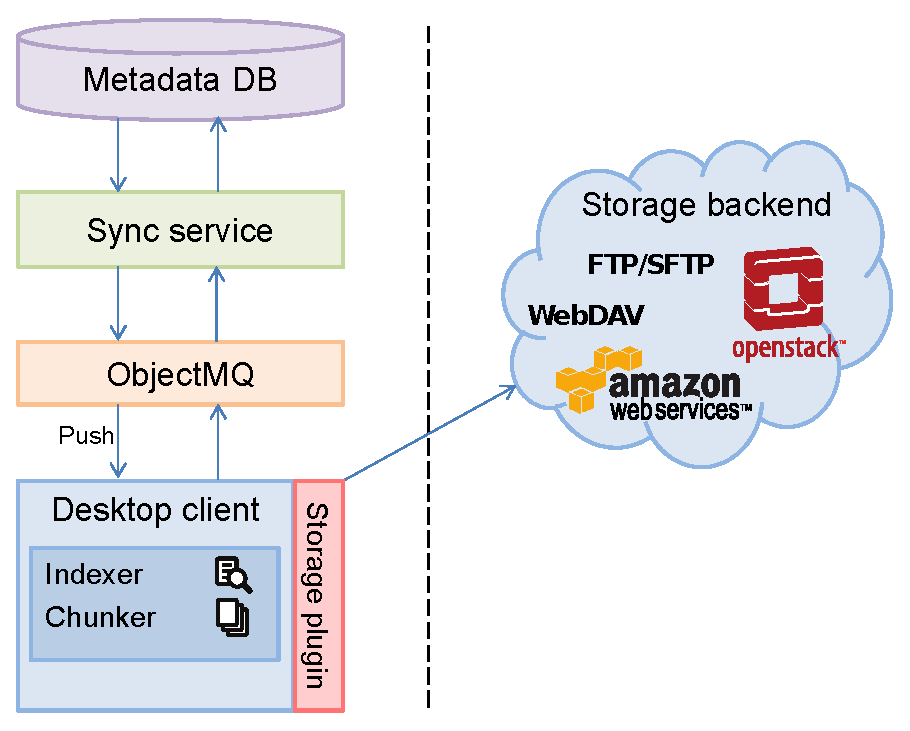
\includegraphics[width=0.55\textwidth]{figures/stacksync_arch_no_api}
\caption{StackSync architecture overview}\label{fig:architecture_no_api}
\end{figure}


As we can see in the figure above, the storage back-end is separated from the rest of the architecture by a line. This means that StackSync can be used with external storage back-ends such as Amazon S3 or RackSpace. This enables StackSync to fit different organization requirements and be offered in three different configurations:

\begin{itemize}
\item \textbf{Public Cloud.} Data and metadata is stored in a public storage provider such as Amazon or Rackspace.
\item \textbf{Private Cloud.} StackSync is installed on-premise. Data and metadata is stored on the company’s infrastructure.
\item \textbf{Hybrid Cloud.} Data is stored in a public storage provider and metadata is kept inside the company’s infrastructure.
\end{itemize}



\subsection{Desktop client and Storage back-ends}

The main StackSync client is a application that monitors local folders and synchronizes them with a remote repository. The StackSync client interacts with both the synchronization and storage services. The first one handles metadata communication, such as time stamps or file names, and the second one is in charge of raw data.


This decoupling of sync control flows from data flows implies a user-centric design where the client directly controls its digital locker or storage container. The synchronization protocol have been designed to put the load in the client side, whereas the synchronization service just
checks if the change is consistent, and then applies all changes proposed by clients.


Every client has a local database and a process called \texttt{Watcher} that is responsible for monitoring the state of local folders that have been selected to be synchronized. If there is any change in the local repository, the \texttt{Watcher} notifies a process called \texttt{Indexer} which is responsible for sending these changes to the synchronization service. Besides that, the \texttt{Indexer} can also receive events from the synchronization service indicating that there was a change in the remote repository. These notifications are applied immediately into the local repository. Regarding potential
conflicts due to offline operations, StackSync provides similar policies than Dropbox, so that we create a copy of the conflicted document and let the user decide about this.


The client uses a chunking algorithm to split files into chunks before they are transmitted to the storage service. To save storage space and bandwidth, the StackSync client uses data deduplication at the chunk level so it only stores and transmits those chunks that have not been uploaded before. 


Finally, and based on the original Syncany architecture, we provide an extensible plugin-based architecture for connecting to third-party Storage back-ends. We now provide plugins for Amazon S3, OpenStack Swift, Dropbox, WebDAV, SMB and FTP. However, we are focusing our efforts on OpenStack Swift, a highly available, distributed, eventually consistent object/blob store that guarantees service scalability.


\subsection{Communication middleware}

StackSync relies on a high-performance message broker compatible with the Advanced Message Queueing Protocol (AMQP)~\cite{amqp} standard. In order to simplify the interaction with this messaging middleware, we have built the ObjectMQ communication middleware.


ObjectMQ is a lightweight remote object layer constructed on top of a messaging
middleware. The current StackSync implementation relies on RabbitMQ~\cite{rabbitmq}, an open source message broker software that implements the AMQP standard. ObjectMQ combines RPC (Remote Procedure Call) and MOM (Message-oriented Middleware) models to devise four MOM-RPC invocation abstractions: two one-to-one calls (synchronous, asynchronous) and two one-to-many calls (multi, event).


In general, objects receive method calls as messages in incoming queues, and then reply the results to clients in response queues. One-to-many calls are distributed using the appropriate AMQP Exchanges (broker message dispatchers). Recall that Exchanges determine message delivery and provide different delivery schemes, like direct (deliver this message to a particular queue) and publish-subscribe (deliver this message to all queues subscribed to a certain topic). 

These are the four available calls:

\begin{itemize}

\item @async:  This is an asynchronous non-blocking  one-way invocation where the client  publishes a message in the target object request 
Queue ($Q_{Request}$). By default, the client expects to receive no response and it is even not notified if the message was handled correctly.


\item @sync:  This is a synchronous blocking remote call where the client publishes a message in the target object
request Queue ($Q_{Request}$), blocking until a response is received in its own client response queue ($Q_{Response}$).  
This call can be configured with a timeout and a number of retries to trigger the exception if the result does not arrive.

\item @event:  This is an asynchronous non-blocking one-to-many notification triggered by a server.  The server triggers an @event by publishing the message in  the Event  fan-out Exchange ($E_{Event}$). Any client subscribing to this event in the server must bind their incoming Event Queue ($Q_{Event}$) to the server Exchange ($E_{Event}$).

\item @multi: This is an asynchronous non-blocking one-to-many invocation from one client to many servers. The clients invokes the method in all servers by publishing an event in the Multi  fan-out Exchange ($E_{Multi}$). All servers bind their incoming Request Queue ($Q_{Request}$) to the Multi Exchange ($E_{Multi}$).
   
\end{itemize}

The ObjectMQ communication middleware supports different compression and transport protocols (Kryo~\cite{kryo}, Java Serialization, JSON). It also handles transparently all the error management and communication services on top of the MOM broker. By creating this middleware, that the initial code of the StackSync client has been reduced in around $3,000$ lines of code.


\subsection{Synchronization service and metadata back-end}

The Sync service is a server-side component implemented as a remote object using the ObjectMQ communication middleware. This service directly benefits from the invocation abstractions offered by ObjectMQ. 

\begin{figure}[t]
\centering
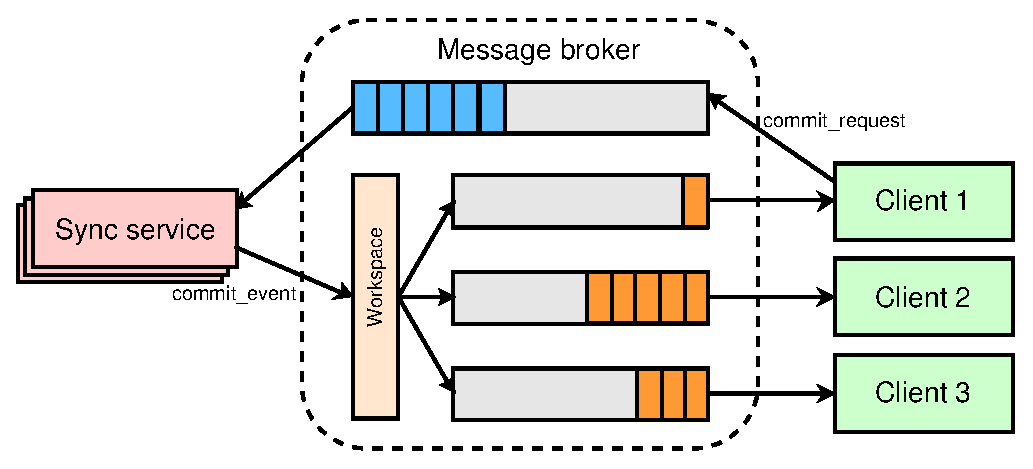
\includegraphics[width=0.66\textwidth]{figures/message_broker}
\caption{Message broker communication flow}\label{fig:message_broker}
\end{figure}


In Figure~\ref{fig:message_broker} we can observe the current design, ObjectMQ is using a global request queue for the SyncService, 
a response queue for each device (Sync service Proxy), and a fan-out Exchange for each workspace.  

Each device will bind its request queue to the appropriate workspace Exchange to receive notification changes in this workspace.  In any case, queue message programming is abstracted thanks to ObjectMQ, so that the protocol will be defined in terms of RPCs or method calls.


\bigskip
\begin{figure}[h!]
	\begin{lstlisting}
	@RemoteInterface
	public interface SyncService extends Remote {

    	@SyncMethod(retry = 5, timeout = 1500)
    	public List<ObjectMetadata> getChanges(Workspace workspace);

    	@SyncMethod(retry = 5, timeout = 1500)
    	public List<Workspace> getWorkspaces();

    	@AsyncMethod
    	public void commitRequest(Workspace workspace, 
    		List<ObjectMetadata> objectsChanged);

	}
	@event
	public interface CommitEvent extends Event {
		
		public List<ObjectMetadata> objectsChanged getChanges();
	}
	
		\end{lstlisting}
		\caption{Sync service interface}
		\label{fig:idl}
\label{Code:push}
\vspace{-10pt}
\end{figure}


In Figure~\ref{fig:idl} we can see the interface definition of the Sync service. Clients can request the list of Workspaces they have access to with the \texttt{getWorkspaces} operation. Once the client obtains the list of Workspaces, it can then perform two main operations: \texttt{getChanges} and  \texttt{commitRequest}. Furthermore, the client will be notified of changes  by means of the event \texttt{CommitEvent}.

\texttt{getChanges} is a synchronous operation (@sync) that StackSync clients perform on startup. This is a costly operation for the Sync service as it returns the current state of a Workspace. Once the client receives this information, it registers its interest in receiving committed updates (i.e. \texttt{CommitEvent}s (@event) for this Workspace). From that point on, any change occurring on this Workspace will be notified to the client in a push style.

\texttt{commitRequest} is an asynchronous operation (@async) that clients employ to inform the Sync service about detected file changes in their Workspaces.  This is a  costly operation since it must guarantee the consistency of data after the new changes. 

\texttt{CommitEvent} is triggered by the Sync service in an asynchronous one-to-many operation (@event) to all out-of-sync devices in the specified Workspace. This operation is only launched by the Sync service once the changes has been correctly stored in the \texttt{Metadata back-end}.

\begin{algorithm}[h]
  \caption{Pseudocode of the commitRequest function in the Sync service}
    \label{alg:commit_pseudocode}
  \begin{algorithmic}[1]
  	\footnotesize
    \Function{commitRequest}{$workspace, List<ObjectMetadata> objects\_changed$}
      \State $commit\_event \gets $ new instance of CommitEvent
      \For{$new\_object$ \textbf{in} $objects\_changed$}
      	\State $server\_object \gets metadata\_backend.get\_current\_version(new\_object.id)$
        \If {\textbf{not exists} $server\_object$}
          	\Comment To commit the first version of the new object
        	\State $metadata\_backend.store\_new\_object(new\_object)$
        	\State $commit\_event.add(new\_object, \mathtt{confirmed} = True)$
        \ElsIf{$server\_object.version$ \textbf{precedes} $new\_object.version$}
         	\\ \Comment No conflict, committing the new version
			\State $metadata\_backend.store\_new\_version(new\_object)$
			\State $commit\_event.add(new\_object, \mathtt{confirmed} =True)$
        \Else
        	\\
        	\Comment Conflict detected, the current object metadata is returned
        	\State $commit\_event.add(new\_object, \mathtt{confirmed} = False,  server\_object)$
        \EndIf
      \EndFor 
      \State $trigger\_event(workspace, commit\_event)$
    \EndFunction
  \end{algorithmic}
\end{algorithm}


Algorithm~\ref{alg:commit_pseudocode} reports the pseudocode of the \texttt{commitRequest} operation. When a \texttt{commitRequest} message is received in the global request queue, the ObjectMQ middleware will invoke the appropriate \texttt{commitRequest} method in the \texttt{SyncService}. 


This method then receives a proposed list of change operations in a concrete Workspace. For every change operation, it will then check if the current version of the object in the \texttt{Metadata back-end} precedes the change proposed by the client. In this case, the changes are (transactionally) stored in the Metadata back-end and confirmed in the \texttt{CommitEvent}. 

If there is a conflict with versions, the \texttt{commitRequest} is set as failed and information about the current object version is added to the \texttt{CommitEvent}. The reason for adding the current object version to the \texttt{CommitEvent} is to piggyback the information about the ``differences'' between the two versions, such that the ``losing'' client can identify the missing chunks and reconstruct the object to the current version. 


In StackSync, a conflict may occur when two users change a file at the same time. This implies that the two clients will propose a list of changes over the same version of the file. The first \texttt{commitRequest} to be processed will
increase the version number by one, but the second \texttt{commitRequest} will inevitably propose a list of changes over a preceding version, resulting in a conflict. 

To resolve the conflict, the Sync service adopts the simplest policy in this case, which is to consider as the ``winner''  the client whose \texttt{commitRequest} was processed first. This way, the Sync service
avoids rolling back any update to the Metadata back-end, saving time and increasing scalability. At the client,
the conflict is resolved by renaming the ``losing'' version of the file to ``...(conflicted copy)''.

Finally, the \texttt{CommitEvent} will be triggered to the Workspace Exchange in message broker, and  it will be received by all interested devices in their incoming event queues. 

Note that the \texttt{CommitRequest} is an important operation in the Sync service since it has to provide scalable request processing, consistency, and scalable change notification. Scalable request processing is achieved because the method is \textit{asynchronous} and \textit{stateless}. Multiple Sync service instances can listen from the global request queue and the message broker will transparently
balance their load. Consistency is achieved using the transactional  ACID model of the underlying Metadata back-end. 
Finally, scalable change notification to the interested parties is achieved using one-to-many push notifications (@event).

The Sync service interacts with the Metadata back-end using an extensible DAO (Data Access Object). Our reference implementation is based on a PostgreSQL relational database although the system is modular and may be replaced easily.


\section{Synchronization Algorithms}

At the core of personal cloud is file sync. Although a rush of online file sync services have
been entering the market during the last years, evidenced by the explosion in popularity of
Dropbox and competitors, little is known about the design and implementation of commercial
sync protocols. According to a recent characterization of Dropbox~\cite{drago2012inside}, file synchronization
is built upon third-party libraries such as librsync, but the role of this library is uncertain
because of the very nature of the rsync algorithm~\cite{tridgell96rsync}. Other popular tools like 
unison~\cite{unison} that use the same basic algorithm suffer from the same deficiencies.

rsync is symmetric, and provides pairwise synchronization between two devices, where the rsync
utility running on each computer must have local access to the entire file. This requirement
poses the first practical limitation to the adoption of rsync because working at the file level
prevents efficient data deduplication. To save storage space and money, services like Dropbox
split files into chunks and store them at multiple nodes on the server side. A straightforward
adaptation of rsync to this context would be piecing together the chunks and reconstructing
whole file at a chosen server and then operate on it. This, unfortunately, would waste massive
intra-cluster bandwidth, deteriorating significantly deduplication efficiency. It is worth
noting here that, although rsync finds chunks of data that occur both in the old file and the
new file, it requires the side acting as a server to compute hashes for all possible alignments
in its file in order to find a match. For this, it needs the whole file.  

In addition, if a single character is modified in each chunk of the old file, then no match
will be found by the server and rsync will be completely useless~\cite{langford01}. To address this limitation,
a number of single-round and multi-round protocols have been proposed in the last ten years. 
Multi-round protocols allow communicating fewer bits in total by using additional communication
rounds; see~\cite{langford01} and~\cite{suel04}. However, the fact of taking multiple passes over files presents evident
disadvantages in terms of protocol complexity, computing and I/O overheads, and communication
latency. Recent single-round protocols~\cite{irmak05}\cite{hao08} bypass this difficulty by using variable-length
content-based chunking~\cite{Muthitacharoen01}. However, since these protocols only synchronize files between two
different machines at a time, they are not directly applicable to Personal Clouds, where file
changes occurring elsewhere are automatically notified to any other device sharing that file. 

There is a large body of work by the OS community that attempts to detect redundancies in order
to reduce storage or transmissions costs, like LFBS~\cite{Muthitacharoen01} and Pastiche~\cite{Cox02}, among others, which
have inspired in one way or another many of today's online cloud storage services. These systems
operate at block level by relying on variable-length content-based chunking, rather than at
file level. Compared with personal cloud applications, distributed file systems pursue a
different objective and can skip implementing some basic functionality in personal clouds like
file version management or the scalable notification of updates as soon as they occur. In fact,
LBFS uses leases in which the server's obligation to inform a client of changes expires after one
minute. The result is that the client will be out of sync once a lease on a file has expired. 
In Dropbox, however, any change on the central storage is advertised as soon as it is made~\cite{drago2012inside}.
For this purpose, the Dropbox client keeps continuously opened a TCP connection to a notification
server, used for receiving information about changes performed elsewhere.

Overall, \textit{providing an efficient and scalable sync protocol} poses a grand challenge for
engineers in charge of building Personal Cloud storage services, due to the intricate
relationships between deduplication, notification and metadata management.
\chapter{Related work}
\section{A Brief History of the Personal Cloud Term}

In the past years there have been divergent views of the ``Personal Cloud'' concept.  
For example, in \cite{hari2012personal} authors propose an architecture and design
for accessing and sharing computational resources in virtual machines. For them, a
Personal Cloud is a collection of Virtual Machines running on unused computers at the edge.
Another different view focuses on collaborative work \cite{ardissono2009service},  
where a web infrastructure is defined to provide a unified environment
for handling activities and collaborations. Finally, a recent trend \cite{windley}
 goes further and defines the Personal Cloud as a cloud Operating 
System that offers a core set of services around identity, trust, data access and 
even programming models.

In this work, we focus on Personal Cloud Storage platforms that take care of data
sync and sharing from heterogeneous devices. In fact,  the term ``Personal Cloud'' have
received a lot of attention with the recent research reports from Forrester \cite{forrester}
and Gartner \cite{gartner}. Like us, these reports associate the term Personal Cloud with
online cloud storage services such as Dropbox, Box, or Google Drive among others.

\section{Synchronization Algorithms}

At the core of Personal Cloud is file sync. Although a rush of online file sync services have
been entering the market during the last years, evidenced by the explosion in popularity of
Dropbox and competitors, little is known about the design and implementation of commercial
sync protocols. According to a recent characterization of Dropbox~\cite{drago2012inside}, file synchronization
is built upon third-party libraries such as librsync, but the role of this library is uncertain
because of the very nature of the rsync algorithm~\cite{tridgell96rsync}. Other popular tools like 
unison~\cite{unison} that use the same basic algorithm suffer from the same deficiencies.

rsync is symmetric, and provides pairwise synchronization between two devices, where the rsync
utility running on each computer must have local access to the entire file. This requirement
poses the first practical limitation to the adoption of rsync because working at the file level
prevents efficient data deduplication. To save storage space and money, services like Dropbox
split files into chunks and store them at multiple nodes on the server side. A straightforward
adaptation of rsync to this context would be piecing together the chunks and reconstructing
whole file at a chosen server and then operate on it. This, unfortunately, would waste massive
intra-cluster bandwidth, deteriorating significantly deduplication efficiency. It is worth
noting here that, although rsync finds chunks of data that occur both in the old file and the
new file, it requires the side acting as a server to compute hashes for all possible alignments
in its file in order to find a match. For this, it needs the whole file.  

In addition, if a single character is modified in each chunk of the old file, then no match
will be found by the server and rsync will be completely useless~\cite{langford01}. To address this limitation,
a number of single-round and multi-round protocols have been proposed in the last ten years. 
Multi-round protocols allow communicating fewer bits in total by using additional communication
rounds; see~\cite{langford01} and~\cite{suel04}. However, the fact of taking multiple passes over files presents evident
disadvantages in terms of protocol complexity, computing and I/O overheads, and communication
latency. Recent single-round protocols~\cite{irmak05}\cite{hao08} bypass this difficulty by using variable-length
content-based chunking~\cite{Muthitacharoen01}. However, since these protocols only synchronize files between two
different machines at a time, they are not directly applicable to Personal Clouds, where file
changes occurring elsewhere are automatically notified to any other device sharing that file. 

There is a large body of work by the OS community that attempts to detect redundancies in order
to reduce storage or transmissions costs, like LFBS~\cite{Muthitacharoen01} and Pastiche~\cite{Cox02}, among others, which
have inspired in one way or another many of today's online cloud storage services. These systems
operate at block level by relying on variable-length content-based chunking, rather than at
file level. Compared with personal cloud applications, distributed file systems pursue a
different objective and can skip implementing some basic functionality in personal clouds like
file version management or the scalable notification of updates as soon as they occur. In fact,
LBFS uses leases in which the server's obligation to inform a client of changes expires after one
minute. The result is that the client will be out of sync once a lease on a file has expired. 
In Dropbox, however, any change on the central storage is advertised as soon as it is made~\cite{drago2012inside}.
For this purpose, the Dropbox client keeps continuously opened a TCP connection to a notification
server, used for receiving information about changes performed elsewhere.

Overall, \textit{providing an efficient and scalable sync protocol} poses a grand challenge for
engineers in charge of building Personal Cloud storage services, due to the intricate
relationships between deduplication, notification and metadata management.

\section{Measurements and benchmarks}
The performance evaluation of Cloud services is a
current hot topic with several papers appearing 
recently~\cite{variability_ccgrid11, nature_data_center_traffic}. A large corpus 
of works have focused on measuring distinct aspects of a Cloud service,
such as computing performance~\cite{ec2benchmarking}, service 
variability~\cite{variability_ccgrid11}, and the nature of 
datacenter traffic~\cite{nature_data_center_traffic}, among
others issues.

Unfortunately, only few works have turned attention to measure the performance
of Cloud storage services. To wit, the authors in~\cite{early_experiences_azure}
explore the performance of Microsoft Azure,
including storage. In this line, the authors in~\cite{s3_grids} execute an extensive
measurement against Amazon S3 to elucidate whether Cloud storage is suitable
for scientific Grids or not.
Similarly, \cite{bergen2011client} presents a performance 
analysis of the Amazon Web Services, with no
insights regarding Personal Clouds.

File hosting and file sharing Cloud services have been analyzed in depth
by several works \cite{imc_rapidshare, one_click_hosting}.
They provide an interesting substrate to understand both
the behavior of users and the QoS of major providers (e.g. RapidShare).

The comparison of public Clouds have recently aroused much
interest. Concretely, the authors in \cite{cloudcmp} present CloudCmp, a systematic
performance and cost comparator of Cloud providers.
The authors validate CloudCmp by measuring the elastic computing, 
storage, and networking services offered by several
public Clouds based on metrics reflecting the impact 
on the performance delivered to customer applications.

In a similar fashion, the authors of \cite{hu2010good} compare Dropbox, Mozy, 
Carbonite and CrashPlan backup services. However, their analysis of 
the performance, reliability and security levels is rather lightweight, and
more work is needed to characterize these services with enough rigor.

Recently, the authors in \cite{drago2012inside} presented an
extensive measurement of DropBox in two scenarios: in a university
campus and in residential networks. They analyzed and characterized the 
traffic transmitted by users, as well as the
functioning and architecture of the service. Instead of analyzing the behavior
of users using a specific Personal Cloud, we focused on
characterizing the service that many providers offer.
\chapter{Measuring Personal Clouds Methodology}

From May $10$, $2012$, to July $15$, $2012$, we installed several
vantage points in our university network (\textit{Universitat
Rovira i Virgili}, Spain) and PlanetLab~\cite{planetlab}  
to measure the performance of three of the major Personal Cloud services in the market: DropBox\footnote{\url{http://www.dropbox.com}}, Box\footnote{\url{http://www.box.net}} 
and SugarSync\footnote{\url{http://www.sugarsync.com}}. The measurement methodology was based on the REST interfaces that these three Personal Cloud storage services provide to developers.

Personal Clouds provide REST APIs, along with
their client implementations, to make it possible for developers to
create novel applications. These APIs incorporate authorization
mechanisms (OAuth~\cite{oauth}) to manage the credentials and tokens
that grant access to the files stored in user accounts. A
developer first registers an application 
in the Cloud provider website and obtains several tokens.
As a result of this process, and once the user has authorized
that application to access his storage space, the Personal Cloud storage service
gives to the developer an \textit{access token}. Including this \textit{access token} in each API call, the application can operate on the user data.

There are two types of API calls: \textit{meta-info} and
\textit{data management} calls. The former type refers to
those calls that retrieve information about the state of the
account (i.e., storage load, filenames), whereas the latter
are those calls targeted at managing the stored files
in the account. %In this work, 
We will analyze the performance
of the most important data management calls: \texttt{PUT} and \texttt{GET},
which serve to store and retrieve files.  


\section{Measurement Platform} 

We employed two different platforms
to execute our tests: University laboratories and PlanetLab.
The reason behind this is that our labs contain
\textit{homogeneous and dedicated machines} that are under our control,
while PlanetLab allows the analysis of each service from \textit{different geographic locations}. 

\textit{University laboratories}. We gathered $30$ machines
belonging to the same laboratory to perform the measurement.
These machines were Intel Core$2$ Duo equipped with $4$GB DDR$2$ RAM. 
The employed operating system was a Debian Linux distribution. 
Machines were internally connected to the same switch via a $100$Mbps Ethernet links.

\textit{PlanetLab}: We collected $40$ PlanetLab nodes divided into
two geographic regions: Western Europe and North America. 
This platform is constituted by heterogeneous (bandwidth, CPU) machines from several
universities and research institutes. Moreover, there were two points to consider
when analyzing data coming from PlanetLab nodes: i) Machines might be concurrently
used by other processes and users, and ii) The quota system of these machines
limited the amount of in/out data transferred daily. 

Specifically, we used the PlanetLab infrastructure for
a high-level assessment of Personal Clouds depending on the 
client's geographic location. 
However, the mechanisms to enforce bandwidth quotas
in PlanetLab nodes may induce the appearance of artifacts 
in bandwidth traces. This made PlanetLab not 
suitable for a fine-grained analysis in our context.
   
\begin{table}%
\begin{center}

\begin{tabular}{|l|l|l|l|}
\hline
Location & Op. Type & Operations & Transferred Data \\ \hline
\multirow{2}{*}{University Labs}
 & \texttt{GET} & $168,396$ & $13.509$ TB\\
 & \texttt{PUT} & $247,210$ & $15.945$ TB\\ \hline
\multirow{2}{*}{PlanetLab}
 & \texttt{GET} & $354,909$ & $31.751$ TB\\
 & \texttt{PUT} & $129,716$ & $9.803$ TB\\ \hline
\end{tabular}
\caption{Summary of Measurement Data (May $10$ $-$ July $15$)}
\vspace{-9mm}
\label{tab:measurement_data}
\end{center}
\end{table}

\section{Workload Model} 

Usually, Personal Cloud services impose file size 
limitations to their REST interfaces, for
we used only files of four sizes to facilitate comparison: $25$MB, $50$MB, 
$100$MB and $150$MB\footnote{Although the official limitation in some cases is fixed
to $300$MB per file, we empirically proved that uploading files
larger than $200$MB is highly difficult. In case of Box this limitation
is $100$MB.}. This approach provides an appropriate substrate 
to compare all providers with a large amount of samples of equal-size files.
Thanks to this, we could observe performance variations of a single provider
managing files of the same size.

In next sections we present the executed worloads.

\subsection{Up/Down Workload}
The objective of this workload
was twofold: Measuring the maximum up/down transfer speed of operations
and detecting correlations between the transfer speed and the load
of an account. Intuitively, the first objective was achieved by alternating upload
and download operations, since the provider only needed to handle one 
operation per account at a time. We achieved the second point
by acquiring information about the load of an account in each API call.

The execution of this workload was continuously performed
at each node as follows: First, a node created synthetic 
files of a size chosen at random from the aforementioned set of sizes.
That node uploaded files until the capacity of the account was full.
At this point, that node downloaded all the files also in random order.
After each download, the file was deleted. 

\subsection{Service Variability Workload}
This workload maintained 
in every node a nearly continuous upload and download transfer flow to analyze the performance 
variability of the service over time. This workload provides an
appropriate substrate to elaborate a time-series analysis of these services.

The procedure was as follows: The upload process first
created files corresponding to each defined file size which
were labeled as ``reserved'', since they were not deleted from the account.
By doing this we assured that the download process was never interrupted,
since at least the reserved files were always ready for being downloaded.
Then, the upload process started uploading synthetic 
random files until the account was full. When the account was full,
this process deleted all files with the exception of the reserved ones
to continue uploading files.
In parallel, the download process was continuously downloading random files
stored in the account. 
 
Finally, we executed the experiments
in different ways depending on the chosen platform. In the case of
PlanetLab, we employed the \textit{same machines in each test}, and therefore, 
we needed to sequentially execute all the combinations of workloads and providers. 
This minimized the impact of hardware and network
heterogeneity, since all the experiments were executed in the same conditions.
On the contrary, in our labs we executed in parallel a certain workload
for all providers (i.e. assigning $10$ machines per provider).
This provided two main advantages: The measurement process was
substantially faster, and fair comparison of the three services
was possible for the same period of time. 
 
We depict in Table \ref{tab:measurement_data} the total 
number of storage operations performed during the measurement period.
\chapter{Benchmarking Personal Clouds Synchronization}

In the evaluation of the reference implementation of StackSync framework, we set out to answer three basic questions: 
$1$) \textit{How much overhead does the system need to support?} $2$) \textit{How much time is needed to have multiple devices in sync?}; and 
$3$) \textit{How does the system internally scale?}

In some of these tests, we compare StackSync against other popular Personal Cloud services, including Dropbox, Microsoft OneDrive, Amazon Cloud Drive, Google Drive and Box.

\section{Benchmark Methodology}

\subsection{Benchmark Platform}

\subsection{Testbed}

For all the experiments, we used the following testbed. The testbed included a front-end server and several desktop 
PCs acting as clients. The front-end was an OpenStack Swift deployment with one proxy node and $4$ storage nodes.  
Unless otherwise noted, the proxy node hosted the \texttt{SyncService}, and the PostgreSQL database acting as the \texttt{Metadata back-end}. Let us review the node specs:
\begin{itemize}
\item Proxy node: Ubuntu $12.04$; Intel Xeon CPU E5-2407; Memory: $12$ GB RAM.
\item Storage nodes: Ubuntu $12.04$;  Intel Xeon CPU E5-2403; Memory: $8$ GB RAM.
\item Desktop PCs: Ubuntu $12.04$; Intel Core i5 2400; Memory: $4$ GB RAM.
\end{itemize}

Tables~\ref{table:services} and~\ref{table:clients} shows the software versions for the services and desktop clients used in the evaluation.

\begin{table}[!htb]
    \begin{minipage}{.5\linewidth}
      \centering
        \begin{tabular}{ | l | l | }
    	\hline
    	Service name & Version \\ \hline
    	OpenStack Swift & \textit{Havana} \\
    	RabbitMQ & 2.8.7 \\
    	PostgreSQL & 9.1 \\
    	SyncService & 0.4.4 \\ \hline
    	\end{tabular}
    \caption{Used services version}
    \label{table:services}
    \end{minipage}%
    \begin{minipage}{.5\linewidth}
      \centering
        \begin{tabular}{ | l | l | }
    	\hline
    	Client name & Version \\ \hline
    	StackSync & 1.6.4 \\
    	Dropbox & 2.6.33 \\
    	Microsoft OneDrive & 17.0.4035.0328 \\
    	Amazon Cloud Drive & 2.4.2013.3290 \\ 
    	Google Drive & 1.15.6430.6825 \\ 
    	Box & 4.0.4925 \\ \hline
    	\end{tabular}
    \caption{Used desktop clients version}
    \label{table:clients}
    \end{minipage} 
\end{table}

\subsection{Setup and Benchmarking Tool}

To evaluate the system, we developed a benchmarking tool to generate
realistic workloads. We implemented this tool because we found no publicly available trace containing both 
the files and the history of modifications to those files that allowed us to evaluate our file-syncing service.

To determine the size of the files, we used the distribution presented in~\cite{liu2013},
a five-month study involving around $20,000$ users. Some of their conclusions
were that the $90\%$ of files are smaller than $4$ MB and that updated files tend to be read sooner
rather than later. Also, they noticed that most of files are read-only.

Imitating the real behavior of users, our tool creates a trace with $3$ different actions: ADD representing the addition
of a file, UPDATE signaling a modification, and REMOVE meaning the removal of the file from the workspace.

In order to determine the action to be performed to a file, we applied the Markov model proposed in~\cite{Tarasov12}. 
In this model, each file can be in $4$ possible states: $\mathtt{N}$ \textemdash~new; $\mathtt{M} $\textemdash~modified; 
$\mathtt{U}$ \textemdash~unmodified; and $\mathtt{D}$ \textemdash~deleted.
For each of those states, a set of probabilities govern the transition to the rest of states.
To set up the transition~probability
matrix, we extracted the transition probabilities from the ``\textit{Homes}'' dataset~\cite{Tarasov12}, 
which is the public trace that most resembles the user behavior in a Personal Cloud service.

To decide how to modify the files, we followed the same approach as in \cite{Tarasov12},
which currently supports $3$ modification types: $\mathtt{B}$ \textemdash~the file is modified in the
beginning by prepending some bytes; $\mathtt{E}$ \textemdash~the file is modified at the end; and $\mathtt{M}$ \textemdash~the
file is modified somewhere in the middle.  As in \cite{Tarasov12}, we also supported
combinations of these patterns, namely $\mathtt{BE}$, $\mathtt{BM}$, and $\mathtt{EM}$. For the transition 
probabilities, we used the change pattern of the ``\textit{Homes}'' dataset: the probability for a $\mathtt{B}$ 
change was of $38\%$; for a $\mathtt{E}$ change was of $8\%$, and for a $\mathtt{M}$ change was of $3\%$. 
The rest of the probability mass was granted to combinations of these changes. We only applied these probabilities
in files smaller than $4$ MB, since more than $90\%$ of the I/O requests are for these files, as just
discussed above.

Our trace generator requires only $3$ parameters: $1$) initial number of files; $2$) number
of training iterations; and $3$) number of snapshots. For our experiments, we set the
initial number of files to $20$, and the number of iterations and snapshots to $5$ and
$100$, respectively. The resulting trace contained $940$ ADDs, $72$ UPDATEs and $228$ REMOVEs.
The ADD operations generated a total data volume of $535.41$ MB whereas the UPDATEs only produced
$\approx 14$ KB. The average file size was of $583$ KB. Fig.~\ref{fig:cdf_files} plots
the CDF of file size for our trace.

Finally, to compare StackSync against other popular Personal Cloud services,
we modified the benchmarking tool developed by Drago et al.~\cite{drago2013benchmarking} to
conduct trace-driven experiments with the output of our generator. More specifically, we adapted
their tool to measure the overhead of the different file syncing protocols under a sequence of
ADD, UPDATE, and DELETE operations using real content.

\begin{figure*}[t]
  \centering
  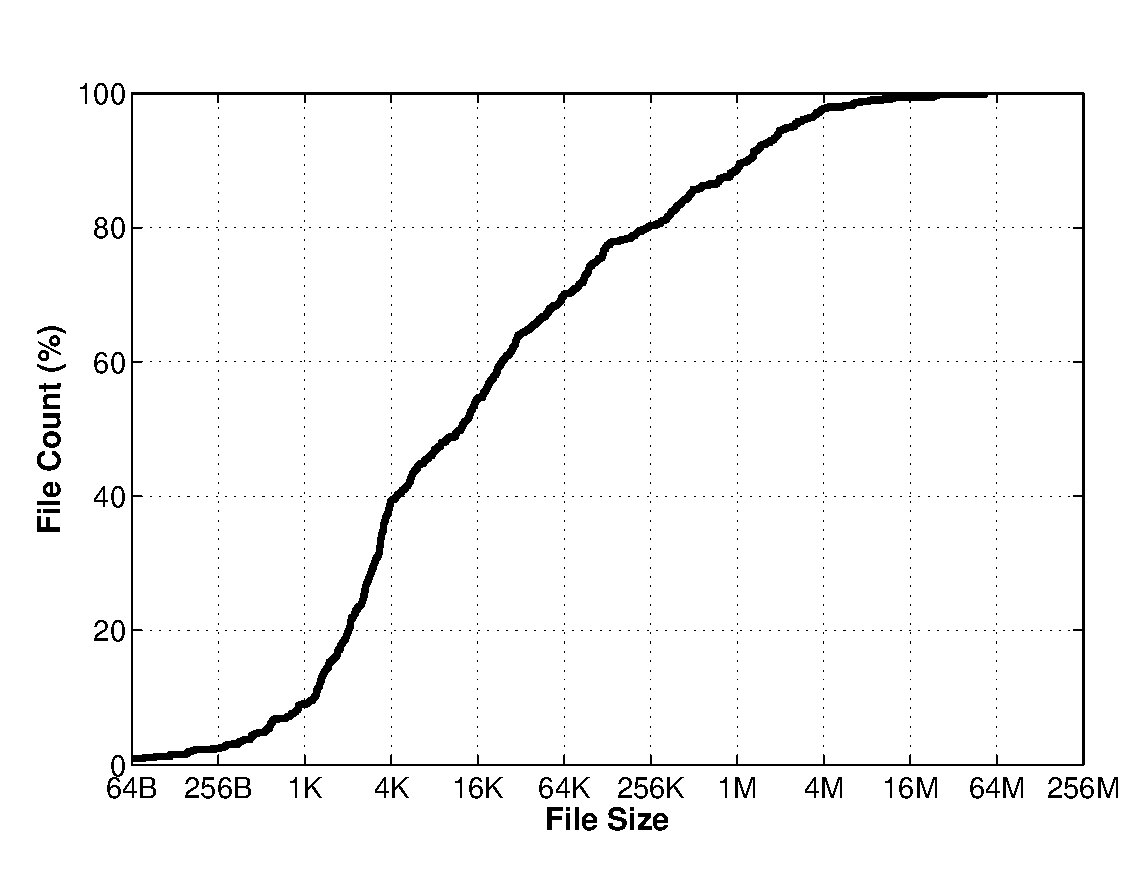
\includegraphics[width=0.7\textwidth]{figures/cdf_files}
  %\vspace{-5pt}
  \caption{File size vs file count distribution}
  \label{fig:cdf_files}
\end{figure*}

\section{Results}

\subsection{Protocol Overhead}
In this test, we compared the protocol overhead of StackSync with the overhead of the
commercial Personal Cloud services reported in Table~\ref{table:clients}. As in~\cite{drago2013benchmarking},
we defined the overhead as the total storage and control traffic over the benchmark size, which was of 
$535.41$ MB. For this experiment, our benchmarking tool considered each of the operations in the trace one at a time,
to measure the overhead accurately. That is, the next operation did not start until the current one was
successfully committed.

\begin{figure*}[h]
  \centering
  \label{fig:overhead_clients}
  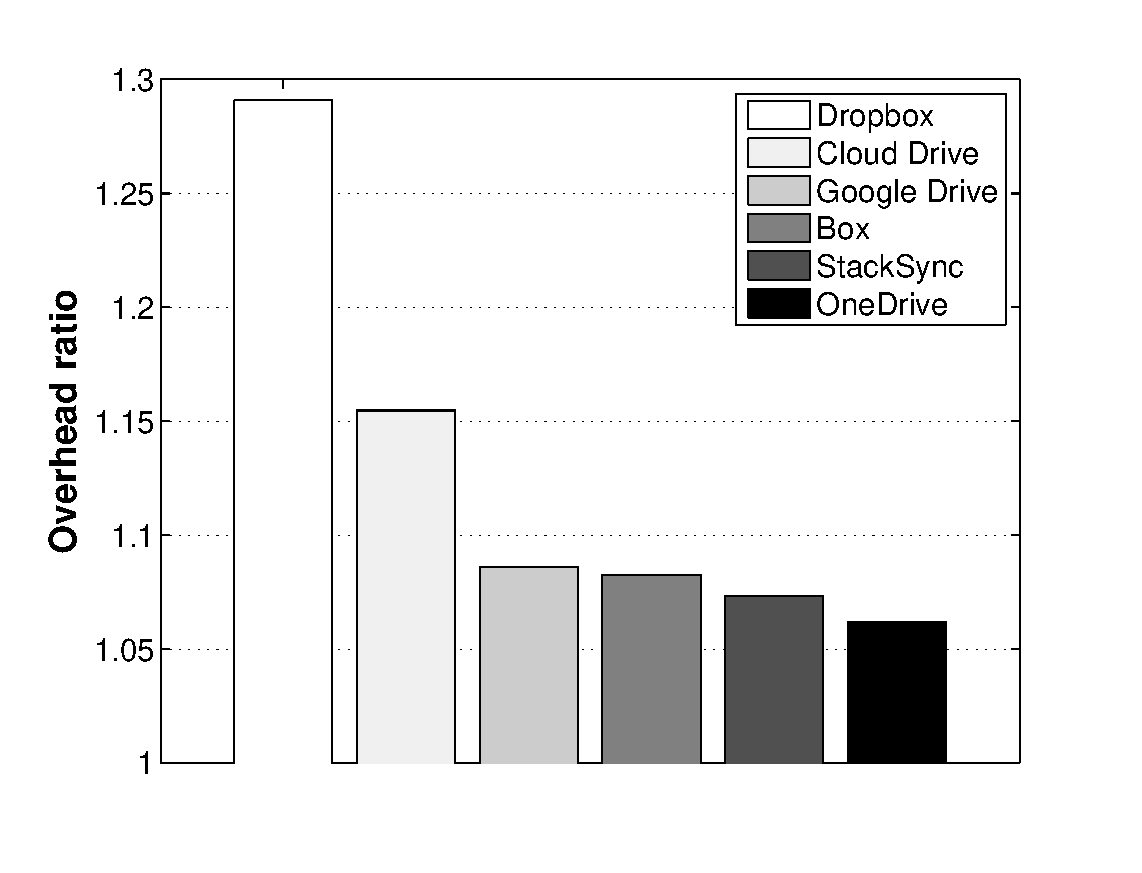
\includegraphics[width=0.6\textwidth]{figures/overhead_clients}
  \caption{Overhead}
\end{figure*}

The results are shown in Fig.~\ref{fig:overhead_clients}. As seen in this
figure, Dropbox exhibits the highest overhead, sending up to $150$ MB of additional
unnecessary traffic. This results agree very well with other studies such as that
of~\cite{liu2013}. On the contrary, StackSync has a low overhead, \textit{comparable to that of commercial
Personal Cloud services such as OneDrive}.


To gain a deeper understanding of the overhead, we prepared a new variant of
this test. In this new variant, we grouped all the actions of the same type to generate $3$ separate traces,
and this way study the overhead per type of action. In this case, we run this experiment only for Dropbox and StackSync
for two main reasons: $1$) because 
Dropbox is the most popular and well-studied Personal Cloud; and $2$) because
it is the Personal Cloud with the highest overhead, which allows for rapid comparison. 
The results are depicted in Fig.\ref{fig:validation:actions_control} for control traffic and Fig.\ref{fig:validation:actions_storage}
for storage traffic.

As shown in Fig.\ref{fig:validation:actions_control}, Dropbox produces a huge amount of control traffic
when adding new files, about $25$ MB of unnecessary traffic, while StackSync only needs $\approx 3.2$ MB.
This indicates that control signaling is significantly much lighter than that of Dropbox. With respect
to storage traffic, StackSync transferred a total amount of $565.63$ MB to the \texttt{Storage back-end},
which is significantly smaller than the $660.32$ MB of storage traffic incurred by Dropbox.

For the UPDATEs, StackSync is negatively affected by the fact that a modification of a few bytes requires to upload at 
least one chunk of  $512$ KB, incurring a huge overhead. Since Dropbox uses delta encoding~\cite{drago2013benchmarking}, a specialized
compression technique, it outperformed StackSinc. It is important to note here that although the 
overhead for StackSync is apparently high, in practice, StackSync transferred only $5$ MB and Dropbox $2$ MB. 
Both values are relatively high compared with the amount of  modified data ($13.50$ KB). 

As the setup of these tests were not favorable to Dropbox, because the actions were performed one after
another without benefiting from the Dropbox file bundling feature, we created a new test that
performs more one action at the same time. Table \ref{table:bundle} lists
the results obtained after executing the trace for both Dropbox and StackSync with different
batch sizes. Dropbox reduces traffic overhead in $30$ MB but it continues to be much higher than the
rest of the Personal Clouds.

\begin{figure*}[t]
  \centering
  \subfigure[Control traffic overhead]{
    \label{fig:validation:actions_control}
    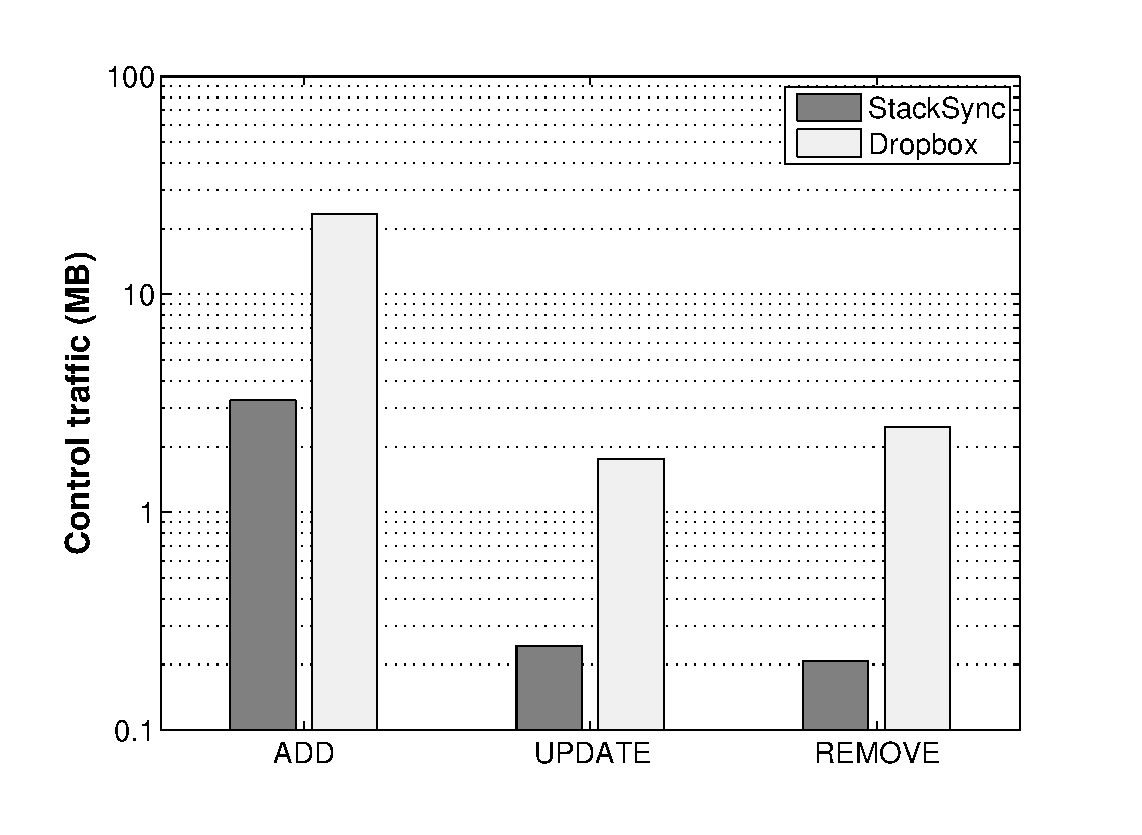
\includegraphics[width=0.45\textwidth]{figures/actions_metadata}
  }
  \subfigure[Storage traffic overhead]{
    \label{fig:validation:actions_storage}
    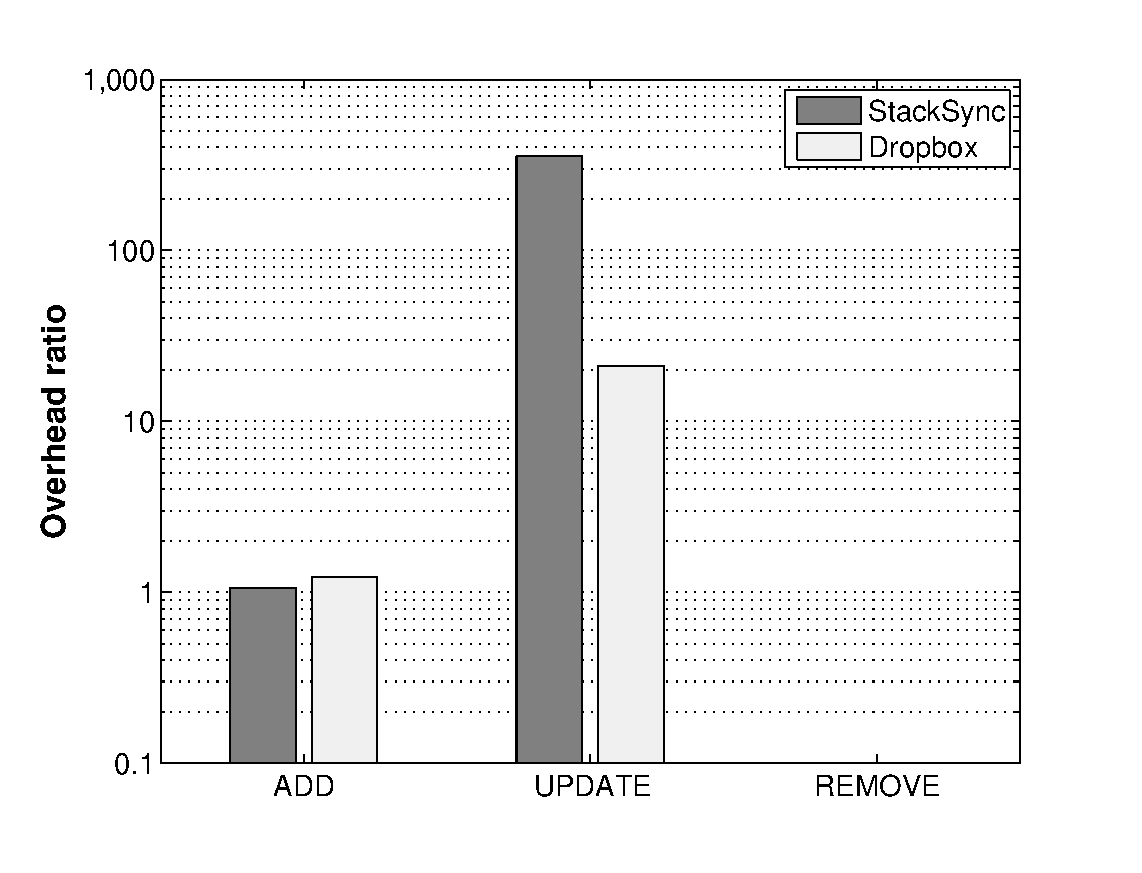
\includegraphics[width=0.45\textwidth]{figures/actions_storage}
  }
  \caption{Control and storage traffic overhead of StackSync and Dropbox}
  \label{fig:validation}
\end{figure*}

\begin{table}
    \centering
    \begin{tabular}{  c | c | c | c | c | }
    \cline{2-5}
    & Batch size & Control & Storage & Total \\ \hline
    \multicolumn{1}{ |c| }{\multirow{4}{*}{Dropbox}} & 5 & 8.30 MB & 633.06 MB & 641.36 MB \\ \cline{2-5}
    \multicolumn{1}{ |c| }{}& 10 & 5.13 MB & 638.26 MB & 643.39 MB \\ \cline{2-5} 
    \multicolumn{1}{ |c| }{}& 20 & 3.28 MB & 635.82 MB & 639.10 MB \\ \cline{2-5}
    \multicolumn{1}{ |c| }{}& 40 & 2.23 MB & 632.05 MB & 634.28 MB \\ \hline
    \multicolumn{1}{ |c| }{\multirow{4}{*}{StackSync}} & 5 & 2.14 MB & 569.89 MB & 572.03 MB \\ \cline{2-5}
    \multicolumn{1}{ |c| }{}& 10 & 1.58 MB & 570.10 MB &  571.68 MB \\ \cline{2-5}
    \multicolumn{1}{ |c| }{}& 20 & 1.37 MB & 570.07 MB & 571.44 MB \\ \cline{2-5}
    \multicolumn{1}{ |c| }{}& 40 & 1.25 MB & 567.77 MB & 569.02 MB \\ \hline
    \end{tabular}
    \caption{Effect of File Bundling.}
    \label{table:bundle}
\end{table} 

\subsection{Synchronization Time}

Another basic question to be examined is the delay experienced~by users to have their devices in sync. 
To answer this question, we measured the time to synchronize $6$ clients for each type
of workspace changes, i.e., ADD, UPDATE and REMOVE. 
The synchronization time was measured as the time elapsed after the modification
was detected by the \texttt{Watcher} of the client that performed it until the local working copies of the other
five clients were in sync. In the case of ADDs and UPDATEs, this time included the delay incurred
to upload and download the unique chunks from the \texttt{Storage back-end}, hosted in our local cluster. 

The results are depicted in Fig.~\ref{fig:synchronization_time:a}. As can be seen in the figure, all the operations take
only a few seconds to have all the clients in sync, even in the case of the ADD operation where an appreciable
amount of time is taken up to access the \texttt{Storage back-end}. Because the REMOVE operation does not trigger any data flow to and from the
\texttt{Storage back-end}, the synchronization time becomes a good estimator of the processing time
incurred by the tandem ObjectMQ-\texttt{SyncService}. 

As shown in the figure, the time to reconcile
a file removal in five clients is less than $2.6$ seconds, which is quite good, assuming that the
\texttt{Metada back-end} is a SQL database.
As a boxplot enables to assess the dispersion of a given distribution, 
we gain important qualitative
insights from Fig.~\ref{fig:synchronization_time:a}. One key observation is that the distribution of the
synchronization time for the UPDATE operation is right skewed, exhibiting file synchronization times
significantly greater than the median value of $2.75$ seconds. This is evidenced~by
the significant number of UPDATE operations exceeding the upper whisker. This skewness is explained
by the use of fixed-size blocks, which suffer from the \textit{boundary shifting problem}~\cite{Eshghi05}.

Since the time taken up by the ADD operation is affected by the file size, one interesting question
is to assess how file size affects the synchronization time. Fig.~\ref{fig:synchronization_time:b} shows the synchronization
time as a function of file size. As can be seen in the figure, \textit{the larger the file size, the longer
the synchronization time}. However, what is most interesting is the fact that the increase in time
is only linear when file size is larger than $2.5$ MBs, which indicates that for small files the
time to transfer chunks from and to the \texttt{Storage back-end} is not significant compared
with the time incurred by the tandem ObjectMQ-\texttt{SyncService}. 

\begin{figure*}[t]
  \centering
  \subfigure[Boxplots of synchronization time]{
    \label{fig:synchronization_time:a}
    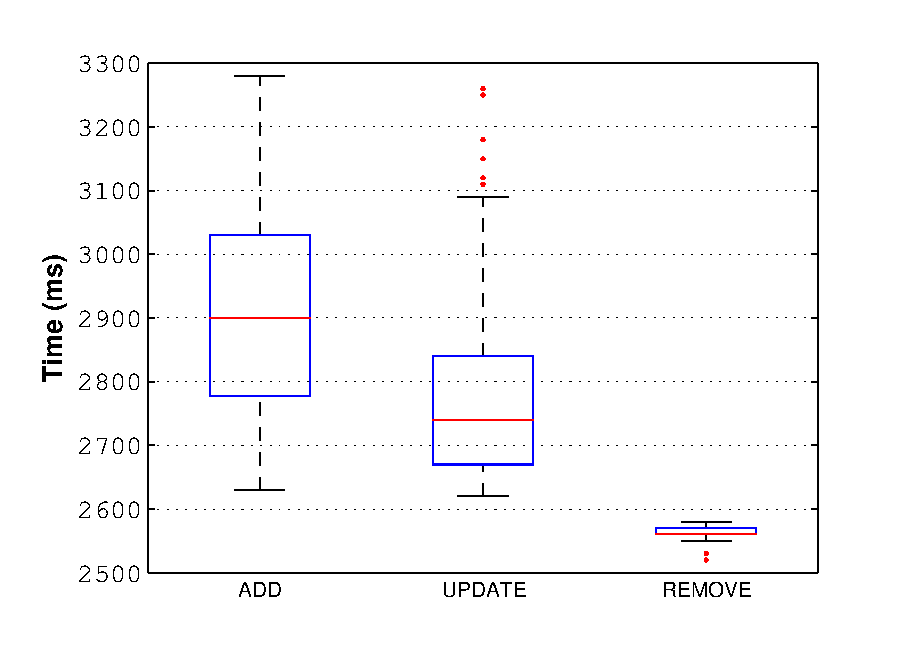
\includegraphics[width=0.45\textwidth]{figures/fig10_2}
  }
  \subfigure[Synchronization time against file size]{
    \label{fig:synchronization_time:b}
    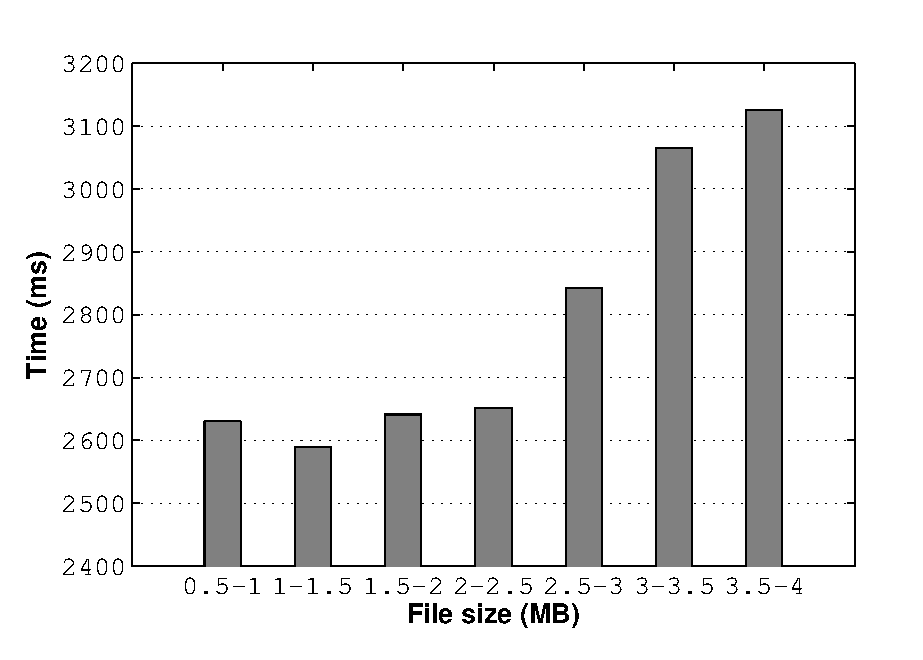
\includegraphics[width=0.45\textwidth]{figures/fig11}
  }
	\caption{Synchronization time}
  \vspace{-5pt}
  \label{fig:synchronization_time}
\end{figure*}


\subsection{Scalability and load-balancing}

Finally, we performed an initial experiment to assess the scalability and load-balancing of 
the StackSync platform. To this end, we performed stress tests generating $100$, $200$, and
$400$ commit requests per second from different clients. We wanted to measure how our service
handles a high number of operations per second, and how the load can be balanced among different
\texttt{SyncService} instances.

In this experiment, we used several system setups: $10$ Desktop PCs generating each one $10$ 
requests per second ($100$ commits/sec in the server), $20$ Desktop PCs generating each one
$10$ requests per second ($200$ commits/sec in the server), and $20$ Desktop PCs generating
each one $20$ requests per second ($400$ commits/sec in the server). 
The used trace was the same of the prior experiments but injected from different clients.
For each system configuration, we executed the experiment using either one single-threaded or four single-threaded 
\texttt{SyncService} instances. 

For each commit request, we recorded the time since the client sent out the commit request until the commit event 
confirming this changes was received in the client. Note that this time captured the entire life-cycle of the protocol,
including message dispatching, time to process the operation in the \texttt{SyncService}
(including access to the database), and finally the dispatching of the commit event to the requesting node.

\begin{figure}[t]
\centering
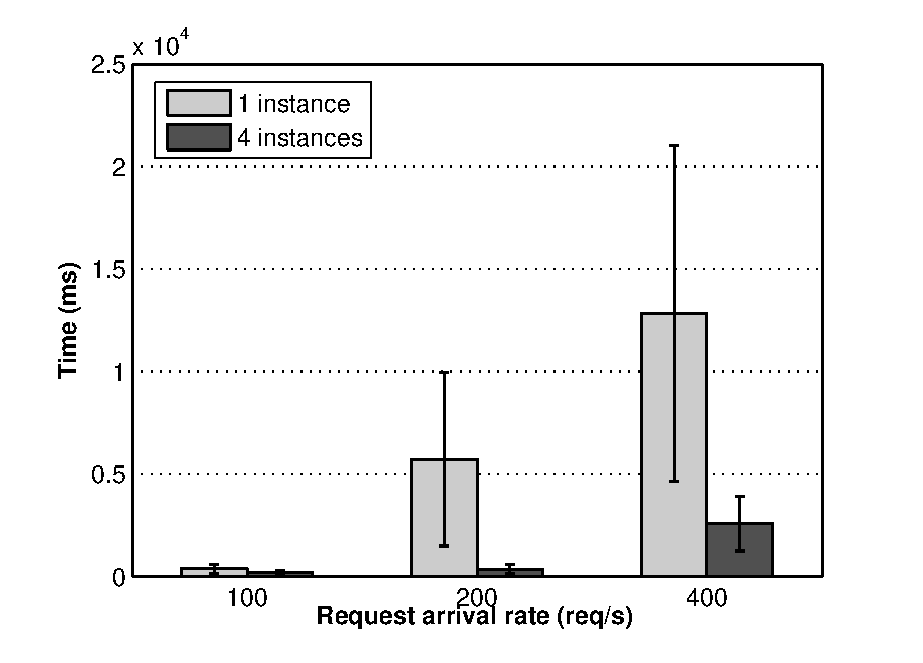
\includegraphics[width=0.5\textwidth]{figures/performance_scalability}
\caption{Scalability and load balancing}\label{fig:scalability}
\end{figure}


In Fig. ~\ref{fig:scalability}, we illustrate the time for $1$ and $4$ \texttt{SyncService}s under different
loads: $100$, $200$, $400$ commits/sec. Our service shows promising numbers in the processing of concurrent
requests since it is able to handle a commit in less than $0.1$ seconds with $4$ instances when receiving
a bulk of $200$ requests/sec. This clearly indicates that balancing the load
among multiple instances produces a significant performance boost. If we consider that all services are
running in the same machine, our results show that the bottleneck is in the transactional database
rather than in the communication layer, i.e., ObjectMQ. The performance gains observed here open the
way to future optimizations to fine tune the scalability of the overall service. 





\subsection{ownCloud Vs StackSync}

In this first experiment we want to compare the metadata overhead produced by ownCloud and StackSync. As stated in the related work, ownCloud is using a pull-based approach based on the WEBDAV protocol. The ownCloud client discover changes by continuously pulling the server with WEBDAV PROPFIND requests for the root user folder every 30 seconds approximately. Each of these requests returns a XML file with a full list of the files and their associated metadata.


Since the PROPFIND request only returns the metadata of the files in the same level, it will not contain change information of files or folders in the levels below. This implies that a change in a subfolder will trigger recursive PROPFIND requests in all the levels of the path. When the change is located in the subfolder, the client then performs a GET request to retrieve the file and stay synced with the rest of the clients.

\begin{figure*}[t]
  \centering
  \subfigure[ownCloud vs StackSync metadata overhead]{
    \label{fig:time:a}
    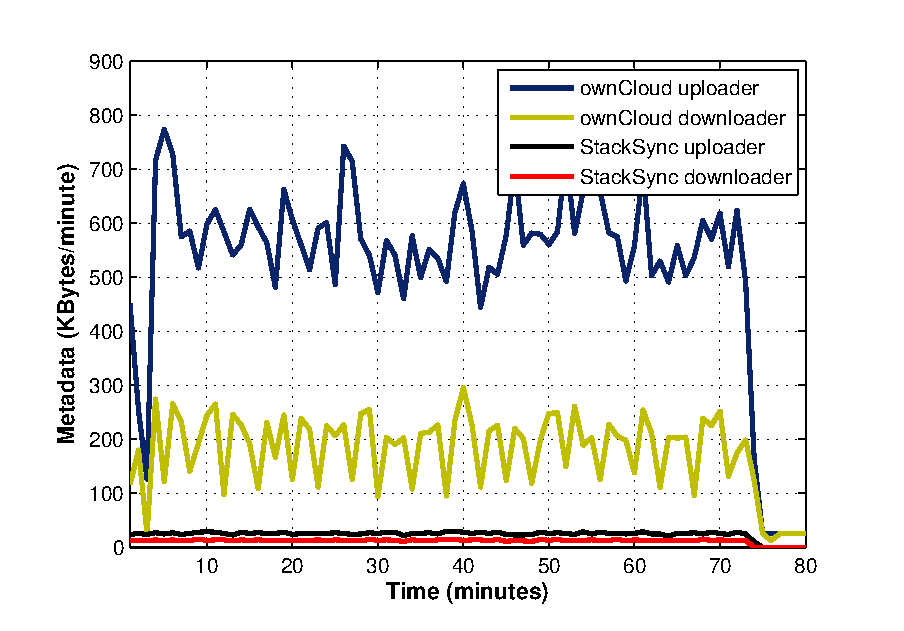
\includegraphics[width=0.45\textwidth]{figures/owncloud_vs_ss_metadata}
  }
  \subfigure[ownCloud sync protocol]{
    \label{fig:time:b}
    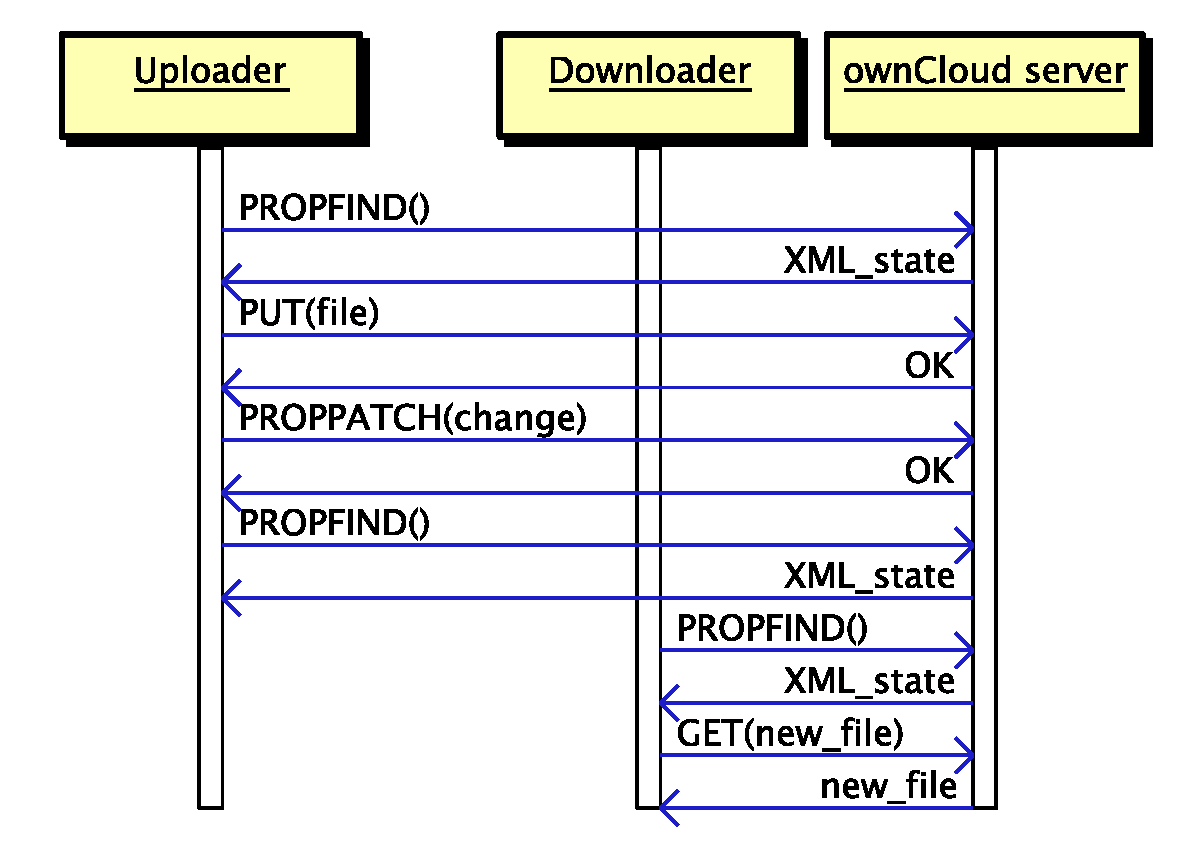
\includegraphics[width=0.45\textwidth]{figures/owncloud}
  }
  \caption{ownCloud vs StackSync}
  \vspace{-5pt}
  \label{fig:owncloud}
\end{figure*}


Due to obvious reasons, this behaviour can be highly inefficient since the amount of metadata exchanged between the server and the client to stay synced could be important (i.e. discover a new file stored in a five-level depth folder produces five PROPFIND requests). It is also important to take into account that each PROPFIND request over a folder involves to get the metadata of all the files inside this folder.

In Fig.~\ref{fig:owncloud} we can see the metadata overhead for ownCloud and StackSync when one node modifies files (uploader) and other must synchronise these changes (downloader). As we can observe in the figure, ownCloud's uploader node is producing for our experiment around 600-800 KBytes/minutes of metadata traffic, and the downloader is producing around 100-300 KBytes/minute of medatada traffic.  This massive traffic is a direct consequence of the inefficient ownCloud pull protocol.

In Fig.~\ref{fig:owncloud} we can see the sequence diagram of ownCloud sync protocol. The node committing new changes (uploader) first obtains the current state (PROPFIND), then uploads the file (PUT), then requests the new change (PROPPATCH), and then rechecks with PROPFIND that the change was correctly applied. The rest of nodes (downloaders) will just ask for changes (PROPFIND) and then retrieve (GET) the entire file. 


Note that PROPFIND and PROPPATCH are synchronous calls that are blocking the client and the server. Note also that if the change is not located in the root folder, it will require recursive PROPFIND requests for the entire path to the change for all clients.  This is not an optimized protocol but a simple pull interface to WEBDAV. As we can see in Fig.~\ref{fig:owncloud},  StackSync is producing an order of magnitude less overhead  than ownCloud for the same experiment  (around 10KBytes/Minute for both uploader and downloader nodes). 


Besides the inefficient metadata processing based on WebDAV pulling, data traffic is coupled to the same metadata server. Furthermore, ownCloud lacks any chunking, deduplication or even caching mechanisms. It just uploads or downloads the entire file if anything has changed.

ownCloud has devoted most efforts in developing the web document manager and web applications. They are providing a very simple and minimalist WEBDAV front-end  to their web server. This could work for a single user (home repository) but the amount of useless traffic make it clearly infeasible for a large deployment.
\chapter{Conclusions}

In this article, we have introduced StackSync, an open framework for Personal Cloud systems.
Its architecture is highly modular, with each module represented by a well-defined API,
allowing researchers to replace components for innovation in versioning,
deduplication, live synchronization or continuous reconciliation, among other relevant topics. 
StackSync provides a reference implementation and useful tools for rapid prototyping and evaluation. 
The reference implementation of the file synchronization engine has been built
on top of a lightweight MOM-RPC middleware, called ObjectMQ, whose one-to-one and one-to-many
abstractions has considerably simplified the design of StackSync. This middleware is ideally
suited to support push notification over persistent connections,
which is critical for live synchronization.  

StackSync is now under active development in the context of the FP7 CloudSpaces project
with the collaboration of several partners. Further work includes adding privacy measures and
supporting adaptive storage in collaboration with EPFL and EURECOM. 
Since today most of these systems are proprietary, relying on infrastructures that are
invisible to the research community, we believe that StackSync will help to advance state
of the art in Personal Cloud systems.

\bibliographystyle{plain}
\bibliography{citations}

% \include{tutorials}

\end{document}
